\documentclass[11pt]{article}
\usepackage[usenames,dvipsnames]{xcolor}
\usepackage{listings}
\usepackage{graphicx}
\usepackage{tikz}
\usetikzlibrary{positioning,backgrounds,fit}
\usepackage{amsmath,amssymb,amsthm,amsfonts} % assumes amsmath package installed
\usepackage[linktocpage=true,colorlinks=true,linkcolor=blue,citecolor=blue,urlcolor=blue]{hyperref}
\usepackage[letterpaper,margin=1in]{geometry}
\usepackage{DejaVuSans}

% \newtheorem{definition}{Definition}
% \newtheorem{assumption}{Assumption}
% \newtheorem{theorem}{Theorem}
% \newtheorem{lemma}{Lemma}
% \newtheorem{proposition}{Proposition}
% \newtheorem{remark}{Remark}

\newcommand{\bx}{\boldsymbol{x}}
\newcommand{\blambda}{\boldsymbol{\lambda}}
\newcommand{\bu}{\boldsymbol{u}}
\newcommand{\bw}{\boldsymbol{w}}
\newcommand{\by}{\boldsymbol{y}}
\newcommand{\bz}{\boldsymbol{z}}
\newcommand{\bV}{\boldsymbol{V}}
\newcommand{\bX}{\boldsymbol{X}}
\newcommand{\bY}{\boldsymbol{Y}}
\newcommand{\bZ}{\boldsymbol{Z}}
\newcommand{\bv}{\boldsymbol{v}}
\newcommand{\bxi}{\boldsymbol{\xi}}
\newcommand{\bpi}{\boldsymbol{\pi}}
\newcommand{\bphi}{\boldsymbol{\phi}}
\newcommand{\bbeta}{\boldsymbol{\eta}}
\newcommand{\bpsi}{\boldsymbol{\psi}}
\newcommand{\bzeta}{\boldsymbol{\zeta}}
\newcommand{\bmu}{\boldsymbol{\mu}}
\newcommand{\bq}{\boldsymbol{q}}
\newcommand{\bQ}{\boldsymbol{Q}}
\newcommand{\bK}{\boldsymbol{K}}
\newcommand{\bP}{\boldsymbol{P}}
\newcommand{\bS}{\boldsymbol{S}}
\newcommand{\bT}{\boldsymbol{T}}
\newcommand{\bF}{\boldsymbol{F}}
\newcommand{\bG}{\boldsymbol{G}}
\newcommand{\bd}{\boldsymbol{d}}
\newcommand{\bp}{\boldsymbol{p}}
\newcommand{\bff}{\boldsymbol{f}}
\newcommand{\bc}{\boldsymbol{c}}
\newcommand{\bg}{\boldsymbol{g}}
\newcommand{\bA}{\boldsymbol{A}}
\newcommand{\bL}{\boldsymbol{L}}
\newcommand{\ba}{\boldsymbol{a}}
\newcommand{\bB}{\boldsymbol{B}}
\newcommand{\bC}{\boldsymbol{C}}
\newcommand{\bE}{\boldsymbol{E}}
\newcommand{\bH}{\boldsymbol{H}}
\newcommand{\bR}{\boldsymbol{R}}
\newcommand{\bn}{\boldsymbol{n}}
\newcommand{\bm}{\boldsymbol{m}}
\newcommand{\br}{\boldsymbol{r}}
\newcommand{\bl}{\boldsymbol{l}}
\newcommand{\bI}{\boldsymbol{I}}
\newcommand{\osigma}{\overline{\sigma}}
\newcommand{\usigma}{\underline{\sigma}}
\newcommand{\oosigma}{\overline{\osigma}}
\newcommand{\uusigma}{\underline{\usigma}}
\newcommand{\olambda}{\overline{\lambda}}
\newcommand{\ulambda}{\underline{\lambda}}
\newcommand{\oolambda}{\overline{\olambda}}
\newcommand{\uulambda}{\underline{\ulambda}}
\newcommand{\bzero}{\boldsymbol{0}}
\newcommand{\st}{\mathop{\text{\normalfont s.t.}}}
\newcommand{\diag}{\mathop{\text{\normalfont diag}}}
\newcommand{\amin}{\mathop{\text{\normalfont argmin}}}
\newcommand{\interior}{\mathop{\text{\normalfont interior}}}
\newcommand{\ReH}{\mathop{\text{\normalfont ReH}}}
\newcommand{\bbZ}{\mathbb{Z}}
\newcommand{\cG}{\mathcal{G}}
\newcommand{\cV}{\mathcal{V}}
\newcommand{\cW}{\mathcal{W}}
\newcommand{\cA}{\mathcal{A}}
\newcommand{\cB}{\mathcal{B}}
\newcommand{\cL}{\mathcal{L}}
\newcommand{\cE}{\mathcal{E}}
\newcommand{\cP}{\mathcal{P}}
\newcommand{\cQ}{\mathcal{Q}}
\newcommand{\cK}{\mathcal{K}}
\newcommand{\cM}{\mathcal{M}}
\newcommand{\cN}{\mathcal{N}}
\newcommand{\cI}{\mathcal{I}}
\newcommand{\cJ}{\mathcal{J}}
\newcommand{\cT}{\mathcal{T}}



% ── Julia syntax highlighting colours ──────────────────────────────────
\definecolor{jlkw}{HTML}{7B3294}      % keywords: purple
\definecolor{jltype}{HTML}{1F78B4}    % types: blue
\definecolor{jlmacro}{HTML}{E31A1C}   % macros: red
\definecolor{jlstr}{HTML}{A6761D}     % strings: brown
\definecolor{jlcmt}{HTML}{636363}     % comments: grey
\definecolor{jlnum}{HTML}{1B7837}     % numbers: dark green
\definecolor{jlbg}{HTML}{F7F7F7}      % background: light grey

% ── Julia language definition for listings ────────────────────────────
\lstdefinelanguage{Julia}{%
  morekeywords={abstract,break,case,catch,const,continue,do,else,elseif,%
    end,export,false,for,function,global,if,import,in,let,local,%
    macro,module,mutable,nothing,quote,return,struct,true,try,%
    type,typealias,using,where,while},
  morekeywords=[2]{Int,Int64,Int32,Float64,Float32,Bool,String,Symbol,%
    Vector,Matrix,Array,Dict,Tuple,NamedTuple,Any,Nothing,Type,%
    AbstractFloat,AbstractArray,AbstractVector,AbstractMatrix,%
    UnitRange,StepRange},
  morekeywords=[3]{@add_var,@add_par,@add_obj,@add_con,@add_con!,%
    @add_expr,@register_univariate,@register_bivariate,%
    @simd,@inbounds,@kernel,@index,@sprintf,@info,@eval},
  sensitive=true,
  alsoother={\$},
  morecomment=[l]\#,
  morecomment=[n]{\#=}{=\#},
  morestring=[s]{"}{"},
  morestring=[m]{'}{'},
}[keywords,comments,strings]

% ── Default listing style ─────────────────────────────────────────────
\lstset{%
  language         = Julia,
  basicstyle       = \small\ttfamily,
  columns          = fullflexible,
  keywordstyle     = \bfseries\color{jlkw},
  keywordstyle     = [2]\color{jltype},
  keywordstyle     = [3]\bfseries\color{jlmacro},
  stringstyle      = \color{jlstr},
  commentstyle     = \itshape\color{jlcmt},
  showstringspaces = false,
  numbers          = left,
  numberstyle      = \scriptsize\ttfamily\color{Gray},
  stepnumber       = 1,
  numbersep        = 8pt,
  tabsize          = 4,
  breaklines       = true,
  backgroundcolor  = \color{jlbg},
  frame            = single,
  rulecolor        = \color{Gray!40},
  framesep         = 3pt,
  xleftmargin      = 2em,
  framexleftmargin = 2em,
  texcl            = true,
  literate         =
    {!=}{{{\color{jlkw}!=}}}2
    {<=}{{{\color{jlkw}<=}}}2
    {>=}{{{\color{jlkw}>=}}}2
    {==}{{{\color{jlkw}==}}}2
    {=>}{{{\color{jlkw}=>}}}2
    {->}{{{\color{jlkw}->}}}2
    {+=}{{{\color{jlkw}+=}}}2
    {0}{{{\color{jlnum}0}}}1
    {1}{{{\color{jlnum}1}}}1
    {2}{{{\color{jlnum}2}}}1
    {3}{{{\color{jlnum}3}}}1
    {4}{{{\color{jlnum}4}}}1
    {5}{{{\color{jlnum}5}}}1
    {6}{{{\color{jlnum}6}}}1
    {7}{{{\color{jlnum}7}}}1
    {8}{{{\color{jlnum}8}}}1
    {9}{{{\color{jlnum}9}}}1,
  % ExaModels-specific identifiers
  emph={ExaCore,ExaModel,ExaModels,Variable,Constraint,Objective,Expression,%
    SIMDFunction,Compressor,NLPModelMeta,CUDABackend,ROCmBackend,%
    NLPModelsIpopt,ipopt,solution,multipliers,set_value!,set_start!,%
    get_start,get_lvar,set_lvar!,get_uvar,set_uvar!,get_lcon,set_lcon!,%
    get_ucon,set_ucon!,get_value,convert_array,replace_T},
  emphstyle=\color{jltype},
}

\providecommand{\keywords}[1]{%
  \small\textbf{\textit{Keywords---}} #1%
}

\definecolor{j1}{rgb}{0.0,0.6056031611752245,0.9786801175696073}
\definecolor{j2}{rgb}{0.8888735002725198,0.43564919034818994,0.2781229361419438}
\definecolor{j3}{rgb}{0.2422242978521988,0.6432750931576305,0.3044486515341153}
\definecolor{j4}{rgb}{0.7644401754934356,0.4441117794687767,0.8242975359232758}
\definecolor{j5}{rgb}{0.6755439572114057,0.5556623322045815,0.09423433626639477}

\usepackage{algorithm}
\usepackage{algpseudocode}
\usepackage{parskip}
\usepackage[font=small,labelfont=bf]{caption}
\usepackage{booktabs}
\usepackage{longtable}
\usepackage[style=authoryear,backend=biber,natbib=true,doi=false,url=false,maxbibnames=999]{biblatex}
\addbibresource{main.bib}
\usepackage[capitalise,noabbrev]{cleveref}
\crefformat{equation}{(#2#1#3)}
\crefrangeformat{equation}{(#3#1#4)--(#5#2#6)}
\crefmultiformat{equation}{(#2#1#3)}{ and (#2#1#3)}{, (#2#1#3)}{ and (#2#1#3)}
\Crefformat{equation}{Equation~(#2#1#3)}
\Crefrangeformat{equation}{Equations~(#3#1#4)--(#5#2#6)}
\Crefmultiformat{equation}{Equations~(#2#1#3)}{ and (#2#1#3)}{, (#2#1#3)}{ and (#2#1#3)}


\title{ExaModels.jl: an Algebraic~Modeling~System for Nonlinear~Programming on GPUs}
\author{Sungho Shin$^*$, Francois Pacaud$^{\dag,\ddag}$, Alexis Montoison$^\ddag$, Michel Schaunen$^\ddag$, Mihai Anitescu$^{\ddag,\S}$}
\date{\small
  $^*$Department of Chemical Engineering, Massachusetts Institute of Technology\\
  $^\dag$MINES Paris - PSL\\
  $^\ddag$Mathematics and Computer Science Division, Argonne National Laboratory\\
  $^\dag$Department of Statistics, University of Chicago\\
}
\begin{document}
\maketitle
\begin{abstract}
  We present ExaModels.jl, an algebraic modeling system for nonlinear programming implemented in Julia. ExaModels.jl is built on a \emph{single-instruction, multiple-data (SIMD) abstraction} that decomposes a nonlinear program into a small number of computational patterns, each evaluated over many data points.
  % SS: decomposes can 
  This pattern--data separation enables three key capabilities: (i) a \emph{parameterized expression tree} whose structure is encoded entirely in the Julia type system, enabling compile-time specialization with no runtime dispatch; (ii) \emph{coloring-free sparse automatic differentiation} that exploits the regular sparsity structure of each pattern to compute exact Jacobians and Hessians without graph coloring; and (iii) \emph{GPU acceleration} via KernelAbstractions.jl, where each pattern becomes a GPU kernel and each data point becomes a thread, achieving high occupancy with no thread divergence. ExaModels.jl implements the NLPModels.jl callback interface and connects to a broad ecosystem of nonlinear programming solvers including Ipopt, KNITRO, MadNLP.jl, and Uno. The system supports parameterized problems, two-stage stochastic programs, and batch optimization. Full type stability enables ahead-of-time compilation to standalone binaries via \texttt{juliac}. We demonstrate the approach on scalable benchmark problems from the Luk\v{s}an--Vlc\v{e}k collection, COPS test suite, and AC optimal power flow instances from PGLIB.
\end{abstract}

\keywords{algebraic modeling system, automatic differentiation, nonlinear programming, parallel computing, GPU computing}

%% ====================================================================
%% OUTLINE — section and subsection structure 
%% ====================================================================

\section{Introduction}
\label{sec:intro}

Large-scale nonlinear programs (NLPs) arising from engineering applications almost always exhibit highly repetitive structure: the same computational pattern appears across many data points in both the objective and constraints. For instance, the alternating current optimal power flow (ACOPF) problem---one of the most widely studied NLPs in power systems---can be expressed with only 15 distinct computational patterns, regardless of whether the network contains hundreds or tens of thousands of buses \cite{shinAcceleratingOptimalPower2024}. Exploiting this repetitive structure is key to efficiently evaluating model functions and their derivatives, which in turn is crucial for the performance of nonlinear optimization solvers. This paper presents a modeling abstraction, an automatic differentiation (AD) algorithm, and their software implementation in ExaModels.jl that exploit this structure and enable GPU acceleration for large-scale NLPs.

To make this concrete, consider the Goddard rocket problem from the COPS benchmark suite \cite{dolanBenchmarkingOptimizationSoftware2001}, discretized via the trapezoidal rule with $T$ time steps:
\begin{subequations}\label{eq:rocket}
\begin{align}
  \max_{h,v,m,\tau,\Delta t} \quad
  & h_T \\
  \st \quad
  & h_t = h_{t-1} + \tfrac{\Delta t}{2}(v_t + v_{t-1}), & t &\in [T], \label{eq:rocket:h}\\
  & v_t = v_{t-1} + \tfrac{\Delta t}{2}\!\left(\frac{\tau_t - D(h_t,v_t)}{m_t} - g(h_t) + \frac{\tau_{t-1} - D(h_{t-1},v_{t-1})}{m_{t-1}} - g(h_{t-1})\right)\!, & t &\in [T], \label{eq:rocket:v}\\
  & m_t = m_{t-1} - \tfrac{\Delta t}{2c}(\tau_t + \tau_{t-1}), & t &\in [T], \label{eq:rocket:m}\\
  & h_0 = h^0,\; v_0 = 0,\; m_0 = m^0,\; m_T = m^f,
\end{align}
\end{subequations}
where $h_t$, $v_t$, $m_t$, and $\tau_t$ are the altitude, velocity, mass, and thrust at time $t$; $D(h,v)$ and $g(h)$ are the aerodynamic drag and gravitational acceleration; and $c$ is the exhaust velocity. When the discretization is refined, the problem size grows proportionally in $T$, but the number of distinct computational patterns---the three dynamics constraints \eqref{eq:rocket:h}--\eqref{eq:rocket:m} and the boundary conditions---remains fixed at five. The model function and derivative evaluations can be naturally expressed as \texttt{for} loops over the time index, and these loops are embarrassingly parallel. Thus, for a modeling system to effectively and concisely express this structure, it should allow users to write their model in a way that preserves the pattern--data separation. A direct consequence is compact model and derivative code that is easier to compile and execute, either on CPUs or GPUs. This observation motivates the following question:
\begin{quote}
  \emph{What modeling abstraction preserves the pattern structure of large-scale NLPs and enables efficient parallel model and derivative evaluation?}
\end{quote}

\paragraph{Algebraic modeling systems.}
An algebraic modeling system (AMS) is a software layer that sits between the user's mathematical formulation and the numerical solver. The user specifies the optimization problem in a high-level syntax, and the AMS translates it into the callback functions---objective, gradient, constraints, Jacobian, Hessian---that the solver requires. This decoupling is central to modern optimization software: the modeling layer and the solver layer are independent modules, and ExaModels.jl is concerned exclusively with the modeling layer. It is \emph{not} a solver; it provides the model information that solvers consume.

Prominent AMSs span a range of problem classes and design philosophies. AMPL \cite{fourerModelingLanguageMathematical1990} is a dedicated modeling language with its own compiler and AD engine, supporting linear, integer, and nonlinear programs. JuMP \cite{lubinJuMP10Recent2023} is an embedded modeling language in Julia that targets a broad class of optimization problems---linear, conic, integer, and nonlinear---through the MathOptInterface (MOI) abstraction layer. CasADi \cite{anderssonCasADiSoftwareFramework2019} is a symbolic framework for algorithmic differentiation, widely used in optimal control and robotics, that generates efficient C code for function and derivative evaluation. Pyomo \cite{hartPyomoModelingSolving2011} is a Python-based framework for mathematical programming that supports a wide range of problem types including stochastic and disjunctive programs. CVXPY \cite{diamondCVXPYPythonEmbeddedModeling2016} is a Python-embedded language for convex optimization based on disciplined convex programming (DCP). Gravity \cite{hijaziGravityMathematicalModeling2018} is a C++-based AMS that introduces ``constraint templates'' to preserve the pattern structure of network optimization problems. Table~\ref{tab:ams} summarizes these systems. We note that ExaModels.jl targets a narrower problem class than most of these systems: we focus exclusively on smooth nonlinear programs (NLPs) as defined in \eqref{eq:nlp}, and do not handle integer variables, conic constraints, or disciplined convex programming constructs.

\begin{table}[!htbp]
  \centering
  \caption{Comparison of algebraic modeling systems. ``Pattern-aware'' indicates whether the system preserves the repetitive structure of the model for SIMD-parallel derivative evaluation.}
  \label{tab:ams}
  \small
  \begin{tabular*}{\textwidth}{@{\extracolsep{\fill}}l l l c c@{}}
    \toprule
    System & Language & Problem classes & AD & Pattern-aware \\
    \midrule
    AMPL & Own language & LP, MILP, NLP & built-in & no \\
    JuMP & Julia (embedded) & LP, MILP, conic, NLP & symbolic & no \\
    CasADi & C++/Python/MATLAB & NLP, OCP & source-generated & no \\
    Pyomo & Python (embedded) & LP, MILP, NLP, stochastic & external & no \\
    CVXPY & Python (embedded) & convex (DCP) & reduction-based & no \\
    Gravity & C++ & NLP (network) & built-in & yes \\
    \midrule
    ExaModels.jl & Julia (embedded) & NLP & built-in & yes \\
    \bottomrule
  \end{tabular*}
\end{table}

\paragraph{Monolithic vs.\ structured representations.}
Most AMSs---including AMPL, JuMP, CasADi, and Pyomo---flatten the model into a monolithic expression graph during the model construction phase. This flattening loses the pattern structure and makes it difficult to apply AD in a single-instruction, multiple-data (SIMD) fashion, which is essential for GPU acceleration. As a result, existing AMSs are not designed to exploit the repetitive structure of large-scale NLPs and generally do not support GPU-based derivative evaluation. Gravity is a notable exception: its ``constraint templates'' preserve the pattern structure, and it has demonstrated excellent AD scalability on ACOPF problems.

\paragraph{Our approach.}
ExaModels.jl adopts a philosophy that is slightly more restrictive than general-purpose AMSs: it \emph{requires} the user to express the model in a structured form where each objective term and constraint is specified as a computational pattern paired with a data iterator. This is a deliberate design choice---by asking the user to expose the parallelizable structure of their problem, ExaModels.jl can exploit it for efficient derivative evaluation. The resulting NLP model information is stored as a collection of patterns and their associated data points. For each pattern, a single derivative evaluation kernel is compiled once and executed across all data points in a SIMD fashion. This is the key to enabling GPU acceleration for large-scale NLPs.

Another key contribution of ExaModels.jl is the \emph{parameterized expression tree}, the core data structure for representing NLP model information. Each expression tree encodes a computational pattern as a type-stable graph of operations, parameterized by problem data supplied at evaluation time. This design allows the expression tree to be evaluated and differentiated with different data and arguments without recompilation---a property that is crucial for GPU execution, where we compile the derivative evaluation kernels once and execute them across many data points.

Furthermore, we implement a novel sparse reverse-mode AD algorithm that does not require graph coloring. This is enabled by an \emph{a priori} sparsity analysis in which the relative index sequence of nonzero entries within each pattern is analyzed at model-construction time and compressed into a compact mapping. This allows us to directly compute the sparse Jacobian and Hessian in coordinate format without the overhead of coloring, which is especially beneficial for GPU execution where dynamic control flow can be costly.

ExaModels.jl provides a convenient user syntax for model construction, including macros for adding variables, parameters, objectives, and constraints, as well as for registering custom functions with their first and second derivatives. Multi-backend GPU execution is supported via KernelAbstractions.jl \cite{churavyKernelAbstractionsjl2025}, allowing users to run on NVIDIA (CUDA), AMD (ROCm), Intel (oneAPI), or Apple (Metal) accelerators without modifying their model code. We demonstrate the performance of ExaModels.jl on a variety of benchmark problems, showing significant speedups over existing AMSs and effective GPU acceleration.

We also provide three extensions that address core use cases for scalable NLPs: \emph{parametric} NLPs, where problem data can be updated without model reconstruction; \emph{two-stage stochastic} programs, with first-stage (design) and second-stage (recourse) variables replicated across scenarios; and \emph{batch} models, where multiple independent NLP instances sharing the same structure are evaluated simultaneously. The underlying SIMD abstraction and AD algorithms apply directly to all three extensions.

ExaModels.jl is implemented in Julia \cite{bezansonJuliaFreshApproach2017}, a just-in-time (JIT) compiled language with a powerful type system and multiple dispatch. The user constructs the model in a high-level syntax, and the underlying data structures and AD algorithms are compiled and optimized for the specific model structure. We leverage Julia's multiple dispatch to enable efficient function registration and maintain type stability throughout the model construction and derivative evaluation process. Importantly, ExaModels.jl is designed to be compatible with ahead-of-time (AOT) compilation via \texttt{juliac} with trimming: it does not rely on runtime code generation or dynamic dispatch in the hot evaluation paths. This makes ExaModels.jl suitable for deployment in production environments where AOT compilation is required, placing it on equal footing with AMSs that feature dedicated code generation, such as CasADi \cite{anderssonCasADiSoftwareFramework2019}.

\paragraph{Contributions.}
In summary, the main contributions of this paper are:
\begin{enumerate}
  \item A SIMD abstraction for modeling large-scale NLPs that preserves the pattern--data structure of the problem.
  \item A parameterized expression tree data structure for efficient, type-stable model storage and evaluation.
  \item A sparse reverse-mode AD algorithm that computes exact Jacobians and Hessians in coordinate format without graph coloring.
  \item A user-friendly modeling syntax with multi-backend GPU support via KernelAbstractions.jl.
  \item Extensions for parametric, two-stage stochastic, and batch NLPs.
  \item Extensive numerical experiments on COPS \cite{dolanBenchmarkingOptimizationSoftware2001}, ACOPF, and Luk\v{s}an--Vlc\v{e}k \cite{lukVsanSparsePartiallySeparable} benchmark problems demonstrating significant speedups over existing AMSs.
\end{enumerate}

\paragraph{Outline.}
The remainder of this paper is organized as follows. Section~\ref{sec:modeling} introduces the modeling abstraction, the SIMD formulation, the core data structures, and the user-facing syntax. Section~\ref{sec:graph} presents the parameterized expression tree. Section~\ref{sec:ad} develops the sparse automatic differentiation algorithm. Section~\ref{sec:gpu} describes GPU acceleration via KernelAbstractions.jl. Section~\ref{sec:aot} addresses type stability and ahead-of-time compilation. Section~\ref{sec:interface} discusses the solver interface. Section~\ref{sec:extensions} introduces the parametric, two-stage, and batch extensions. Section~\ref{sec:numerics} reports numerical experiments. Section~\ref{sec:conclusions} concludes the paper.

\paragraph{Notation.}
We use $[N] := \{1,\ldots,N\}$ for index sets and $\mathbb{R}^n$ for $n$-dimensional real space. Decision variables are denoted $x \in \mathbb{R}^n$ with bounds $x^\flat \leq x \leq x^\sharp$; dual variables (Lagrange multipliers) are $\blambda \in \mathbb{R}^m$. The parameter vector is $\theta$. In the SIMD formulation \eqref{eq:simd}, $f^{(\ell)}$, $g^{(m)}$, $h^{(n)}$ denote computational patterns with associated data collections $\mathcal{D}_\ell$, and $p$, $q$, $s$ denote data points within those collections. Gradients $\nabla f$ are column vectors; the Jacobian $\nabla g$ has dimensions $m \times n$ with rows $\nabla g_j^\top$. Code identifiers are typeset in \texttt{monospace}.

\section{Modeling Abstraction}
\label{sec:modeling}

\subsection{Nonlinear Programming and Algebraic Modeling Systems}
\label{sec:modeling:nlp}

We consider the standard nonlinear program (NLP):
\begin{equation}\label{eq:nlp}
  \min_{x \in \mathbb{R}^n}\; f(x) \quad
  \st\quad g^\flat \leq g(x) \leq g^\sharp,\quad x^\flat \leq x \leq x^\sharp,
\end{equation}
where $f:\mathbb{R}^n \to \mathbb{R}$ is the objective function, $g:\mathbb{R}^n \to \mathbb{R}^m$ is the constraint function, and $x^\flat, x^\sharp, g^\flat, g^\sharp$ are the variable and constraint bounds. Interior-point methods \cite{wachterImplementationInteriorpointFilter2006,nocedalNumericalOptimization2006} and other NLP solvers require the following five callbacks from the modeling layer:
\begin{subequations}\label{eq:callbacks}
\begin{align}
  &\texttt{NLPModels.obj}(m, x) & &\to\; f(x) \in \mathbb{R}, \label{eq:cb:obj}\\
  &\texttt{NLPModels.grad!}(m, x, \nabla\!f) & &\to\; \nabla f(x) \in \mathbb{R}^n, \label{eq:cb:grad}\\
  &\texttt{NLPModels.cons!}(m, x, c) & &\to\; g(x) \in \mathbb{R}^m, \label{eq:cb:cons}\\
  &\texttt{NLPModels.jac\_coord!}(m, x, v) & &\to\; \nabla g(x) \in \mathbb{R}^{m \times n} \;\text{(sparse)}, \label{eq:cb:jac}\\
  &\texttt{NLPModels.hess\_coord!}(m, x, \blambda, v) & &\to\; \nabla^2 f(x) + \textstyle\sum_{j=1}^m \lambda_j \nabla^2 g_j(x) \in \mathbb{R}^{n \times n} \;\text{(sparse)}, \label{eq:cb:hess}
\end{align}
\end{subequations}
where $m$ is the model object. These callbacks follow the NLPModels.jl\footnote{\url{https://github.com/JuliaSmoothOptimizers/NLPModels.jl}} interface developed by the JuliaSmoothOptimizers (JSO) organization. NLPModels.jl defines the abstract type \texttt{AbstractNLPModel} and a standardized callback API that decouples the modeling layer from the solver layer: any model that implements this interface can be used with any solver in the JSO ecosystem, including Ipopt (via NLPModelsIpopt.jl), MadNLP.jl \cite{shinMadNLPjl2025}, Percival.jl, DCISolver.jl, and others. The \texttt{!}-suffixed callbacks write their result into a preallocated output array. The Jacobian and Hessian are stored in coordinate (COO) format---triplets $(r, c, v)$ of row indices, column indices, and values---since the sparsity structure is fixed across solver iterations and only the values $v$ change. The efficiency of these five callbacks dominates the per-iteration cost of the solver, and a key goal of any AMS is to provide them as efficiently as possible.

The role of an algebraic modeling system (AMS) is to bridge the gap between the user's mathematical formulation and these solver callbacks. The AMS provides: (i) a user-facing syntax for expressing the model, (ii) an internal representation (typically an expression graph) for storing the model, (iii) automatic differentiation for evaluating derivatives, and (iv) sparsity detection for constructing the sparse Jacobian and Hessian structures. Established AMSs include AMPL \cite{fourerModelingLanguageMathematical1990}, JuMP \cite{lubinJuMP10Recent2023}, CasADi \cite{anderssonCasADiSoftwareFramework2019}, and Pyomo \cite{hartPyomoModelingSolving2011}.

A common design pattern across these systems is that the model is \emph{flattened} into a monolithic expression graph during construction. That is, each scalar constraint and objective term is recorded as an individual node in a single large graph. While this approach is general and flexible, it discards the repetitive structure present in most engineering models. As a consequence, the AD engine must traverse the entire graph without knowledge of which subexpressions share the same computational pattern, precluding SIMD-parallel derivative evaluation.

\subsection{SIMD Abstraction of Nonlinear Programs}
\label{sec:modeling:simd}

To address this limitation, we adopt a structured representation of NLPs in which the repetitive patterns are explicitly preserved. Specifically, we consider NLPs of the form:
\begin{subequations}\label{eq:simd}
\begin{align}
  \min_{x^\flat \leq x \leq x^\sharp}\;
  & \sum_{\ell \in [L]} \sum_{i \in [I_\ell]} f^{(\ell)}(x;\, p_i^{(\ell)}) \label{eq:simd:obj}\\
  \st\; & g^\flat \leq
  \left[ g^{(m)}(x;\, q_j^{(m)}) \right]_{j \in [J_m]}
  + \sum_{n \in [N_m]} \sum_{k \in [K_n]} h^{(n)}(x;\, s_k^{(n)})
  \leq g^\sharp,
  \quad \forall\, m \in [M], \label{eq:simd:con}
\end{align}
\end{subequations}
where $x \in \mathbb{R}^{n}$ is the vector of decision variables with bounds $x^\flat, x^\sharp$; $f^{(\ell)}$, $g^{(m)}$, and $h^{(n)}$ are twice-differentiable scalar functions referred to as \emph{computational patterns}; and $p_i^{(\ell)}$, $q_j^{(m)}$, $s_k^{(n)}$ are problem data that parameterize each pattern instance. We use $[N] := \{1,\ldots,N\}$ to denote index sets.

The objective \eqref{eq:simd:obj} is decomposed into $L$ groups of objective patterns, where pattern $f^{(\ell)}$ is evaluated over $I_\ell$ data points. The constraints \eqref{eq:simd:con} consist of $M$ blocks: within block $m$, the ``base'' pattern $g^{(m)}$ defines $J_m$ constraints, and the ``augmentation'' patterns $h^{(n)}$ contribute additive terms to these constraints. This augmentation structure arises naturally in network models (e.g., summing arc flows into nodal balance equations) and is discussed further in Section~\ref{sec:data:core}.

The key observation is that many large-scale NLPs arising from engineering applications can be expressed in the form \eqref{eq:simd} with a small number of distinct patterns, even when the problem involves millions of variables and constraints. The Goddard rocket problem \eqref{eq:rocket} is a direct instance: the three dynamics constraints \eqref{eq:rocket:h}--\eqref{eq:rocket:m} are three patterns each evaluated over $T$ data points, and the four boundary conditions contribute four single-instance patterns, giving $L + M = 5$ patterns in total regardless of $T$. The ACOPF model requires only 15 patterns \cite{shinAcceleratingOptimalPower2024}---generation cost, power flows, voltage limits, power balance, and generator/line contributions---regardless of network size. More broadly, the formulation \eqref{eq:simd} captures the full range of COPS benchmark problems \cite{dolanBenchmarkingOptimizationSoftware2001}: optimal control problems (rocket steering, robot arm, hang glider), PDE-constrained optimization (minimal surface, elastic--plastic torsion, journal bearing), parameter estimation with collocation (catalyst mixing, gas--oil yield, marine population dynamics), and mesh/shape optimization (tetrahedral/triangular mesh smoothing, largest polygon, cam shape design). In all of these, the number of distinct patterns is small and fixed, while the problem size scales with the discretization resolution. This \emph{pattern--data separation} is the foundation of the SIMD abstraction.

Because each pattern evaluation is independent across data indices, the derivative computations inherit the same embarrassingly parallel structure. For a given pattern $f^{(\ell)}$, the gradient contributions $\nabla_x f^{(\ell)}(x; p_i^{(\ell)})$ for $i \in [I_\ell]$ can be evaluated in parallel, as can the Hessian contributions. This is in contrast to monolithic expression graphs, where the AD engine must traverse the full graph sequentially (or rely on graph coloring to identify parallelism after the fact). By preserving the pattern structure at the modeling level, ExaModels.jl makes this parallelism directly available to the AD implementation.

In ExaModels.jl, each computational pattern is compiled into a \texttt{SIMDFunction} that provides a per-data-point callback $\tilde{f}(i, x, \theta)$, where $i$ is a data point, $x$ is the decision variable vector, and $\theta$ is the parameter vector. The global objective, for instance, is evaluated as
\begin{equation}\label{eq:simdfunction}
  f(x) = \sum_{\ell \in [L]} \sum_{i \in \mathcal{D}_\ell} \tilde{f}^{(\ell)}(i,\, x,\, \theta),
\end{equation}
where $\mathcal{D}_\ell$ is the data collection associated with pattern $\ell$. The constraints, gradient, Jacobian, and Hessian callbacks follow the same structure: for each pattern, a single compiled kernel is applied across all data points in its collection. The model is therefore stored as a collection of \texttt{SIMDFunction}s---one per pattern---together with their associated data.

Concretely, each \texttt{SIMDFunction} bundles: (i) the parameterized expression tree $\tilde{f}$ (Section~\ref{sec:graph}), (ii) compressor maps for the Jacobian and Hessian that translate the AD traversal into sparse coordinate indices (Section~\ref{sec:ad:sparsity}), and (iii) integer offsets and strides that locate this pattern's contributions within the global output arrays. Given these offsets, each callback in \eqref{eq:callbacks} reduces to a loop over patterns, where each pattern's \texttt{SIMDFunction} is evaluated across all its data points---an embarrassingly parallel operation that maps directly to a GPU kernel (Section~\ref{sec:gpu}). The \texttt{SIMDFunction} is constructed once during model compilation and is immutable thereafter; updating the decision variables $x$ or the parameters $\theta$ requires no recompilation.

% \section{Core Data Structures} — merged into Section 2
\label{sec:data}

We now introduce the two central data structures in ExaModels.jl: \texttt{ExaCore}, the mutable accumulator used during model construction, and \texttt{ExaModel}, the immutable compiled model that implements the NLPModels.jl callback interface.

Both types follow a Julian design pattern: they are \emph{parametric structs} whose type parameters encode the floating-point type \texttt{T}, the array type \texttt{VT}, the backend \texttt{B}, and the concrete types of all stored objectives, constraints, and variables. For example, \texttt{ExaCore\{Float64, Vector\{Float64\}, Nothing, ...\}} represents a CPU model in double precision, while \texttt{ExaCore\{Float32, CuArray\{Float32\}, CUDABackend, ...\}} represents a single-precision model on an NVIDIA GPU. Because these choices are captured as type parameters, Julia's compiler specializes all downstream code---model construction, AD passes, and solver callbacks---for each concrete combination. A single codebase thus handles CPU, CUDA, ROCm, oneAPI, and Metal backends without runtime dispatch or conditional branching.

\subsection{ExaCore: Incremental Model Construction}
\label{sec:data:core}

An \texttt{ExaCore} object serves as the workspace in which the user incrementally builds an optimization model. It is created with a call to \texttt{ExaCore()} (optionally specifying a GPU backend), and the user then adds variables, parameters, objectives, and constraints one at a time via the macros \texttt{@add\_var}, \texttt{@add\_par}, \texttt{@add\_obj}, and \texttt{@add\_con}. Each call appends a new entry to the appropriate tuple stored in the core and updates internal counters. The key fields of \texttt{ExaCore} are:
\begin{itemize}
  \item \texttt{var} --- a tuple of \texttt{Variable} structs, each recording the variable's dimensions, offset into the global variable vector $x$, name, and tag.
  \item \texttt{par} --- a tuple of parameter arrays, whose values are concatenated into the global parameter vector $\theta$.
  \item \texttt{obj} --- a tuple of \texttt{Objective} structs. Each objective stores a \texttt{SIMDFunction} (the compiled pattern) and the collected data iterator.
  \item \texttt{cons} --- a tuple of \texttt{Constraint} and \texttt{ConstraintAugmentation} structs. A \texttt{Constraint} defines a new block of constraints with bounds; a \texttt{ConstraintAugmentation} (created via \texttt{@add\_con!}) adds terms to an existing constraint block without introducing new rows.
  \item Running counters: \texttt{nvar}, \texttt{ncon}, \texttt{nobj}, and the nonzero counts \texttt{nnzj} (Jacobian) and \texttt{nnzh} (Hessian), which are accumulated as patterns are added.
  \item Primal and dual arrays: \texttt{x0}, $\theta$, \texttt{lvar}, \texttt{uvar}, \texttt{y0}, \texttt{lcon}, \texttt{ucon}.
  \item \texttt{backend} --- the KernelAbstractions.jl backend (e.g., \texttt{CUDABackend()}) or \texttt{nothing} for CPU execution.
\end{itemize}
Because each \texttt{@add\_obj}/\texttt{@add\_con} call constructs a \texttt{SIMDFunction} eagerly---probing sparsity and building compressor maps at the time the pattern is registered---the \texttt{ExaCore} accumulates all the information needed for the final model. The tuples \texttt{var}, \texttt{obj}, and \texttt{cons} grow heterogeneously: each entry has a different concrete type (reflecting a different expression tree type), so they are stored as Julia tuples rather than arrays.

\subsection{ExaModel: The Compiled NLP Model}
\label{sec:data:model}

Once all variables, objectives, and constraints have been added, the user calls \texttt{ExaModel(c)} to compile the \texttt{ExaCore} into an immutable \texttt{ExaModel}. This compilation step:
\begin{enumerate}
  \item Constructs the \texttt{NLPModelMeta} object, which stores the problem dimensions ($n$, $m$), initial primal and dual iterates ($x_0$, $y_0$), variable and constraint bounds ($x^\flat$, $x^\sharp$, $g^\flat$, $g^\sharp$), bound classification indices (free, lower-bounded, upper-bounded, fixed), and the nonzero counts \texttt{nnzj} and \texttt{nnzh}. This metadata follows the NLPModels.jl specification and is queried by solvers to allocate sparse structures and select algorithmic options.
  \item Transfers the \texttt{var}, \texttt{par}, \texttt{obj}, and \texttt{cons} tuples from the core, together with the parameter vector $\theta$.
  \item Builds a backend-specific extension (\texttt{ext}) when a GPU backend is active (e.g., pre-allocating device-side workspace arrays).
  \item Initializes an \texttt{NLPModels.Counters} object to track callback invocations during the solve.
\end{enumerate}
The resulting \texttt{ExaModel} is a subtype of \texttt{NLPModels.AbstractNLPModel\{T,VT\}}, where \texttt{T} is the floating-point type and \texttt{VT} is the array type (\texttt{Vector\{T\}} for CPU, \texttt{CuArray\{T\}} for CUDA, etc.). This means it can be passed directly to any solver in the JuliaSmoothOptimizers ecosystem---including Ipopt (via NLPModelsIpopt.jl) and MadNLP.jl \cite{shinMadNLPjl2025}---without any adapter code. The solver calls the five callbacks \eqref{eq:callbacks}, and ExaModels.jl dispatches each callback to a loop over the stored \texttt{SIMDFunction}s.

\subsection{Internal Data Types}
\label{sec:data:internal}

Before describing the user-facing syntax, we briefly describe the internal types that connect the data structures of this section to the expression trees of Section~\ref{sec:graph} and the AD machinery of Section~\ref{sec:ad}.

\paragraph{AbstractNode and expression trees.}
Every mathematical expression in ExaModels.jl is represented as a tree of \texttt{AbstractNode} subtypes. A node is callable as \texttt{node(i, x, $\theta$)}: given a data point~$i$, a primal vector~$x$, and a parameter vector~$\theta$, it returns a scalar value. Interior nodes (\texttt{Node1}, \texttt{Node2}) store a function and references to their children; leaf nodes (\texttt{Var}, \texttt{DataIndexed}, \texttt{Constant}, \texttt{DataSource}) provide access to variables, data, compile-time constants, and the data-point sentinel, respectively. The full node hierarchy and tree construction mechanism are described in Section~\ref{sec:graph}.

\paragraph{SIMDFunction.}
A \texttt{SIMDFunction\{F,C1,C2\}} bundles the compiled representation of a single computational pattern. It contains:
\begin{itemize}
  \item \texttt{f::F} --- the parameterized expression tree (an \texttt{AbstractNode}).
  \item \texttt{comp1::C1}, \texttt{comp2::C2} --- \texttt{Compressor} mappings for Jacobian and Hessian sparsity (Section~\ref{sec:ad:sparsity}).
  \item Offset and stride integers (\texttt{o0}, \texttt{o1}, \texttt{o2}, \texttt{o1step}, \texttt{o2step}) that locate this pattern's entries within the global constraint, Jacobian COO, and Hessian COO arrays.
\end{itemize}
The \texttt{SIMDFunction} is the central compilation artifact: it is constructed at model-construction time by probing the expression tree for sparsity and building the compressor maps, and it is the unit of work for both CPU loops and GPU kernels (Section~\ref{sec:gpu}).

\paragraph{Objective, Constraint, and ConstraintAugmentation.}
Each entry in the \texttt{obj} and \texttt{cons} tuples of an \texttt{ExaCore}/\texttt{ExaModel} is one of three wrapper types:
\begin{itemize}
  \item \texttt{Objective\{F,I\}} --- wraps a \texttt{SIMDFunction} \texttt{f} and a collected data iterator \texttt{itr}. Corresponds to one objective pattern $\tilde{f}^{(\ell)}$ in \eqref{eq:simd:obj}.
  \item \texttt{Constraint\{F,I,O,S,T\}} --- wraps a \texttt{SIMDFunction}, a data iterator, an offset into the global constraint vector, dimension information, and a tag. Corresponds to one base constraint pattern $\tilde{g}^{(m)}$ in \eqref{eq:simd:con}.
  \item \texttt{ConstraintAugmentation\{F,I,D,T\}} --- wraps a \texttt{SIMDFunction} whose expression tree is a \texttt{Pair\{index\_expr, value\_expr\}}. The index expression determines \emph{which} constraint row to augment, and the value expression provides the additive term. Corresponds to the augmentation patterns $\tilde{h}^{(n)}$ in \eqref{eq:simd:con}.
\end{itemize}
This three-type design keeps the number of expression trees minimal. To see why \texttt{ConstraintAugmentation} is essential, consider the active power balance constraint in ACOPF:
\begin{equation*}
  \sum_{g \in \mathcal{G}_b} p_g - p^d_b = \sum_{(b,j) \in \mathcal{E}} p_{bj}  + \sum_{(j,b) \in \mathcal{E}} p_{jb}, \quad \forall b \in \mathcal{B},
\end{equation*}
where $\mathcal{G}_b$ is the set of generators at bus $b$, and $p_{bj}$, $p_{jb}$ are the power flows on lines incident to $b$. Each bus has a different number of generators and incident lines, so the full expression cannot be written as a single parameterized tree evaluated over buses---the tree \emph{structure} varies from bus to bus, violating the SIMD requirement that all data points share the same tree.

With \texttt{@add\_con!}, the problem decomposes cleanly:
\begin{lstlisting}
@add_con(c, -pd[i] for i in bus_data)           # base: one row per bus
@add_con!(c, con[b] += pg[i] for i in gen_data) # generator injection
@add_con!(c, con[b] += pf[i] for i in line_from)# line flow (from end)
@add_con!(c, con[b] += pt[i] for i in line_to)  # line flow (to end)
\end{lstlisting}
Each \texttt{@add\_con!} call creates a separate \texttt{ConstraintAugmentation} with its own fixed-structure expression tree, evaluated over its own data collection (generators, from-lines, to-lines). The augmentation mechanism accumulates all contributions into the correct constraint rows at evaluation time. Without it, the user would need to construct one monolithic expression per bus that inlines every generator and line contribution---destroying the pattern--data separation and preventing SIMD/GPU parallelism.

More broadly, \texttt{@add\_con!} arises naturally whenever a constraint sums over heterogeneous sets. In ACOPF, reactive power balance has the same structure; in optimal control on networks, nodal flow balance constraints are analogous. The augmentation mechanism ensures that the number of distinct patterns scales with the number of \emph{types of contributions} (generator, line-from, line-to), not with the number of constraints or the network topology.

\subsection{User-Facing Syntax}
\label{sec:data:syntax}

This section provides a concise overview of the modeling API. For a complete reference---including all function signatures, keyword arguments, and usage examples---we refer the reader to the online documentation.\footnote{\url{https://exanauts.github.io/ExaModels.jl/stable/}}

The following macros constitute the user-facing API for building an \texttt{ExaCore}:
\begin{itemize}
  \item \texttt{@add\_var(c, x, dims; start, lvar, uvar)} --- creates a variable block \texttt{x} with the given dimensions and optional initial values and bounds.
  \item \texttt{@add\_par(c, p, data)} --- registers a parameter array whose values are concatenated into $\theta$.
  \item \texttt{@add\_obj(c, expr for i in data)} --- adds an objective pattern.  The generator body is the expression tree; the iterator is the data collection $\mathcal{D}$.
  \item \texttt{@add\_con(c, expr for i in data; lcon, ucon)} --- adds a constraint pattern that defines a new block of $|\mathcal{D}|$ constraints with bounds.
  \item \texttt{@add\_con!(c, con[j] += expr for (j, ...) in data)} --- augments an existing constraint block \texttt{con} with additive terms.  This corresponds to the $h^{(n)}$ terms in \eqref{eq:simd:con} and is critical for keeping the number of expression trees small: in network models, each contribution type (e.g., generator injection, line flow) becomes its own pattern rather than being inlined into a single monolithic expression per constraint.
  \item \texttt{@add\_expr(c, expr for i in data)} --- creates a reusable subexpression that can appear in subsequent objectives or constraints.
\end{itemize}
To illustrate the end-to-end workflow, the following code builds and solves the Goddard rocket problem \eqref{eq:rocket} from the introduction:
\begin{lstlisting}
using ExaModels, NLPModelsIpopt

nh = 200                               # number of time steps
h_0, v_0, m_0, g_0 = 1.0, 0.0, 1.0, 1.0
T_c, h_c, v_c, m_c  = 3.5, 500.0, 620.0, 0.6
c_e = 0.5*sqrt(g_0*h_0); m_f = m_c*m_0
D_c = 0.5*v_c*(m_0/g_0); T_max = T_c*m_0*g_0

core = ExaCore(minimize = false)        # maximize final altitude
@add_var(core, h, 0:nh; start = 1.0, lvar = 1.0)
@add_var(core, v, 0:nh; start = (i/nh*(1-i/nh) for i=0:nh))
@add_var(core, m, 0:nh;
  start = ((m_f-m_0)*i/nh + m_0 for i=0:nh), lvar = m_f, uvar = m_0)
@add_var(core, T, 0:nh; start = T_max/2, lvar = 0.0, uvar = T_max)
@add_var(core, step, 1; start = 1/nh, lvar = 0.0)

@add_obj(core, h[nh])                  # objective: final altitude
@add_con(core, c1,                     # altitude dynamics
  -h[i]+h[i-1] + 0.5*step[1]*(v[i]+v[i-1]) for i=1:nh)
@add_con(core, c2,                     # velocity dynamics
  -v[i]+v[i-1] + 0.5*step[1]*(
    (T[i] - D_c*v[i]^2*exp(-h_c*(h[i]-h_0))/h_0
      - m[i]*g_0*(h_0/h[i])^2)/m[i]
    + (T[i-1] - D_c*v[i-1]^2*exp(-h_c*(h[i-1]-h_0))/h_0
      - m[i-1]*g_0*(h_0/h[i-1])^2)/m[i-1]) for i=1:nh)
@add_con(core, c3,                     # mass dynamics
  -m[i]+m[i-1] + 0.5*step[1]*(-T[i]/c_e - T[i-1]/c_e) for i=1:nh)
@add_con(core, bc,                     # boundary conditions
  h[0]-h_0; v[0]-v_0; m[0]-m_0; m[nh]-m_f)

model = ExaModel(core)                 # compile: ExaCore -> ExaModel
result = ipopt(model)                  # solve via Ipopt
\end{lstlisting}
The five patterns (\texttt{c1}--\texttt{c3} dynamics, boundary conditions, and the objective) directly correspond to the mathematical formulation \eqref{eq:rocket}. The same model runs on a GPU by replacing the first line with \texttt{core = ExaCore(minimize = false, backend = CUDABackend())}; no other changes are needed.

\paragraph{Getters, setters, and solution access.}
After the model is built, the user can query and modify bounds, initial points, and parameters:
\begin{lstlisting}
get_start(model, h)              # initial values for h
set_start!(model, h, ones(nh+1)) # update initial values
get_lvar(model, T)               # lower bounds on T
set_lvar!(model, T, zeros(nh+1)) # update lower bounds
\end{lstlisting}
After solving, the solution is accessed per variable and constraint block:
\begin{lstlisting}
h_sol = solution(result, h)      # primal: altitude trajectory
v_sol = solution(result, v)      # primal: velocity trajectory
lam   = multipliers(result, c2)  # dual: velocity dynamics multipliers
\end{lstlisting}
These per-block accessors use the offset and dimension information stored in each \texttt{Variable} and \texttt{Constraint} struct to extract the relevant slice without copying. For parametric models, the parameter values can be updated without model reconstruction via \texttt{set\_value!(model, p, new\_vals)}, since the expression tree structure and all compiled AD code remain unchanged---only the data in $\theta$ is modified.

\section{Parameterized Expression Tree}
\label{sec:graph}

The parameterized expression tree is the core data structure in ExaModels.jl for representing computational patterns. Each objective, constraint, and reusable subexpression in the model is stored as a single expression tree that is \emph{parameterized} by the data supplied at evaluation time. Unlike conventional expression graphs that store one tree per scalar expression, a single parameterized expression tree represents an entire family of expressions---one for each data point in the pattern---enabling the SIMD evaluation and differentiation described in Section~\ref{sec:modeling:simd}.

\subsection{Node Types}
\label{sec:graph:nodes}

An expression tree is a directed acyclic graph whose nodes are subtypes of \texttt{AbstractNode}. Every node is callable as \texttt{node(i, x, $\theta$)}, where $i$ is the data point (iterator element), $x$ is the primal variable vector, and $\theta$ is the parameter vector. The return value is a scalar. The node types fall into two categories.

The node types are:
\begin{itemize}
  \item \textbf{Leaf nodes} supply inputs:
    \texttt{Var\{I\}} evaluates to a decision variable $x[i]$ (with index $i$ that can be a literal or a data-dependent node);
    \texttt{DataIndexed\{I,J\}} evaluates to a field of the data point, with the access path encoded in the type parameters for zero-overhead lookup;
    \texttt{ParameterNode\{I\}} evaluates to a parameter $\theta[i]$;
    \texttt{Constant\{T\}} embeds a compile-time constant as a type parameter (Section~\ref{sec:graph:constants}).
    Real numbers appearing as literal coefficients are handled directly as \texttt{Real} values in binary node children.
  \item \textbf{Interior nodes} compose operations:
    \texttt{Node1\{F,I\}} evaluates as $F(\texttt{inner}(i, x, \theta))$ for a unary function $F$ (e.g., \texttt{sin}, \texttt{exp});
    \texttt{Node2\{F,I1,I2\}} evaluates as $F(\texttt{inner1}(i, x, \theta),\, \texttt{inner2}(i, x, \theta))$ for a binary function $F$ (e.g., $+$, $*$, \texttt{/}).
\end{itemize}

\paragraph{Example.}
To illustrate, consider the extended Rosenbrock objective from the Luk\v{s}an--Vlc\v{e}k benchmark \cite{lukVsanSparsePartiallySeparable}:
\begin{equation}\label{eq:rosenbrock}
  \min_{x \in \mathbb{R}^N}\; \sum_{i=2}^{N} \bigl[100(x_{i-1}^2 - x_i)^2 + (x_{i-1} - 1)^2\bigr].
\end{equation}
In ExaModels.jl, this is specified as a single objective pattern:
\begin{lstlisting}
@add_obj(c, 100*(x[i-1]^2 - x[i])^2 + (x[i-1] - 1)^2 for i in 2:N)
\end{lstlisting}
To understand how a single expression tree is constructed for this pattern, consider what happens when the macro evaluates the generator body. The variable \texttt{x} returned by \texttt{@add\_var} is a \texttt{VarSource} sentinel---not a numeric array, but an object whose \texttt{getindex} method returns symbolic \texttt{Var} nodes. Similarly, the iterator variable \texttt{i} is bound to a \texttt{DataSource} sentinel whose \texttt{getindex}, \texttt{getproperty}, and \texttt{iterate} methods return \texttt{DataIndexed} nodes that encode the access path as type parameters. These overloaded methods extend Julia's standard \texttt{Base.getindex}, \texttt{Base.getproperty}, and \texttt{Base.indexed\_iterate}, allowing the data iterator to supply tuples, named tuples, or nested structures---each field access is captured symbolically in the type.

The tree is built step by step through multiple dispatch. When the generator body is evaluated with these sentinels:
\begin{enumerate}
  \item \texttt{i - 1} dispatches to \texttt{-(::DataSource, ::Int)}, returning a \texttt{DataIndexed} node;
  \item \texttt{x[i-1]} dispatches to \texttt{getindex(::VarSource, ::DataIndexed)}, returning \texttt{Var\{DataIndexed\{...\}\}};
  \item \texttt{x[i-1]\^{}2} dispatches to \texttt{\^{}(::AbstractNode, ::Constant\{2\})}, applying the simplification rule $(\cdot)^2 \to \texttt{abs2}(\cdot)$ and returning a \texttt{Node1\{abs2,...\}};
  \item the subtraction, outer square, multiplication by 100, and addition each dispatch similarly, constructing \texttt{Node2} nodes.
\end{enumerate}
No loop is unrolled: the final result is a single expression tree whose \texttt{Var} leaves resolve variable indices from the data point at evaluation time. The same tree is evaluated for each $i \in \{2,\ldots,N\}$, with different data producing different variable indices and hence different function values and derivatives. This is the ``parameterized'' aspect: a single compiled tree serves all $N-1$ data points, which is the key to SIMD evaluation and GPU acceleration.

Figure~\ref{fig:tree} shows the expression tree for this pattern. Interior nodes (circles) carry their operation as a type parameter; leaf nodes (rectangles) supply inputs. Each \texttt{Var} node (blue) contains a subtree that computes the variable index from the data point $i$: the reference \texttt{x[i-1]} becomes \texttt{Var\{Node2\{+, DataIndexed, Int\}\}}, where the \texttt{DataIndexed} node extracts the integer $i$ from the data point and the \texttt{Node2\{+\}} adds the offset. At evaluation time, this resolves to $x[i + \text{offset}]$, so the same tree evaluates $100(x_1^2 - x_2)^2 + (x_1 - 1)^2$ when $i = 2$, $100(x_2^2 - x_3)^2 + (x_2 - 1)^2$ when $i = 3$, and so on.

\begin{figure}[t]
\centering
\begin{tikzpicture}[
  scale=0.82, transform shape,
  % Uniform rounded-rectangle style for all nodes, color-coded by role
  nd/.style={rectangle, rounded corners=3pt, draw=gray!60, thick, fill=white,
    minimum height=7mm, minimum width=10mm, inner sep=2pt, font=\footnotesize\ttfamily},
  ndvar/.style={nd, draw=j1!80, fill=j1!10},
  nddata/.style={nd, draw=j3!80, fill=j3!10},
  ndconst/.style={nd, draw=j4!70, fill=j4!8},
  ndsrc/.style={nd, draw=j2!80, fill=j2!10},
  % Edge style
  edge from parent/.style={draw, gray!60, semithick},
  % Level spacing
  level 1/.style={sibling distance=58mm, level distance=13mm},
  level 2/.style={sibling distance=30mm, level distance=13mm},
  level 3/.style={sibling distance=22mm, level distance=13mm},
  level 4/.style={sibling distance=17mm, level distance=13mm},
  level 5/.style={sibling distance=14mm, level distance=12mm},
  level 6/.style={sibling distance=14mm, level distance=11mm},
  % Type annotation style
  typelabel/.style={font=\tiny\sffamily, text=gray!60, inner sep=1pt},
]

% Main expression tree
\node[nd] (root) {$+$}
  child { node[nd] (times) {$\times$}
    child { node[ndconst] (c100) {100} }
    child { node[nd] (sq1) {abs2}
      child { node[nd] (sub1) {$-$}
        child { node[nd] (sq2) {abs2}
          child { node[ndvar] (v1) {Var}
            child { node[nd] (plus1) {$+$}
              child { node[nddata] (di1) {$[\,]$}
                child { node[ndsrc] (ds1) {DataSource} }
              }
              child { node[ndconst] (off1) {$o_1$} }
            }
          }
        }
        child { node[ndvar] (v2) {Var}
          child { node[nd] (plus2) {$+$}
            child { node[nddata] (di2) {$[\,]$}
              child { node[ndsrc] (ds2) {DataSource} }
            }
            child { node[ndconst] (off2) {$o_2$} }
          }
        }
      }
    }
  }
  child { node[nd] (sq3) {abs2}
    child { node[nd] (sub2) {$-$}
      child { node[ndvar] (v3) {Var}
        child { node[nd] (plus3) {$+$}
          child { node[nddata] (di3) {$[\,]$}
            child { node[ndsrc] (ds3) {DataSource} }
          }
          child { node[ndconst] (off3) {$o_1$} }
        }
      }
      child { node[ndconst] (c1) {1} }
    }
  };

% Type annotations
\node[typelabel, above right=-1pt and 3pt of root] {Node2\{$+$\}};
\node[typelabel, above right=-1pt and 3pt of sq1] {Node1\{abs2\}};
\node[typelabel, above left=-1pt and 3pt of v1] {Var\{Node2\{$+$,...\}\}};
\node[typelabel, left=3pt of c100, anchor=east] {Constant\{100\}};
\node[typelabel, below=1pt of di1, anchor=north west] {\color{j3!80}DataIndexed};

% Dashed box around a Var subtree to highlight index computation
\begin{scope}[on background layer]
  \node[draw=j1!40, dashed, rounded corners=5pt, fill=j1!3,
    inner sep=4pt, fit=(v1)(plus1)(di1)(off1)(ds1)] {};
\end{scope}

% Semantic annotations: what each subtree evaluates to
\node[font=\tiny\itshape, text=j1!80, anchor=east] at ([xshift=-2pt]v1.west) {$x[i{+}o_1]\leftarrow$};

% Legend — clean horizontal bar
\node[anchor=north, font=\footnotesize, inner sep=0pt] at (0,-9.5) {
  \begin{tikzpicture}[scale=0.82, transform shape]
    \node[nd, minimum size=5mm] at (0,0) {};
    \node[font=\scriptsize, anchor=west] at (0.4,0) {Node1/Node2};
    \node[ndvar, minimum size=5mm] at (2.8,0) {};
    \node[font=\scriptsize, anchor=west] at (3.2,0) {Var};
    \node[nddata, minimum size=5mm] at (4.5,0) {};
    \node[font=\scriptsize, anchor=west] at (4.9,0) {DataIndexed};
    \node[ndconst, minimum size=5mm] at (7.3,0) {};
    \node[font=\scriptsize, anchor=west] at (7.7,0) {Constant};
    \node[ndsrc, minimum size=5mm] at (9.5,0) {};
    \node[font=\scriptsize, anchor=west] at (9.9,0) {DataSource};
  \end{tikzpicture}
};
\end{tikzpicture}
\caption{Parameterized expression tree for the Rosenbrock pattern $100(x_{i-1}^2 - x_i)^2 + (x_{i-1} - 1)^2$. All nodes are uniformly represented as rounded rectangles, color-coded by role. Each \texttt{Var} node (blue) contains a subtree that computes the variable index: the \texttt{DataSource} sentinel (orange) feeds into a \texttt{DataIndexed} node (green) that extracts the data-point index $i$, and the \texttt{Node2\{+\}} adds a compile-time offset $o_k$. The dashed box highlights this index-computation subtree; at runtime, \texttt{Var} evaluates to $x[i + o_k]$, so the same tree serves all $N{-}1$ data points. The simplification $(\cdot)^2 \to \texttt{abs2}(\cdot)$ is applied at construction time. The entire tree structure---including all offsets---is encoded in a single nested Julia type, enabling compile-time specialization.}
\label{fig:tree}
\end{figure}

\subsection{Expression Type and Structure}
\label{sec:graph:type}

The type of a parameterized expression tree is worth discussing explicitly, as it is the mechanism that enables compile-time specialization.

Each node type is parameterized by the types of its children. A \texttt{Node1\{F,I\}} encodes not only the function $F$ but also the full type \texttt{I} of its child subtree. A \texttt{Node2\{F,I1,I2\}} similarly encodes both child types. Since the leaf types carry their own type parameters (\texttt{Var\{I\}}, \texttt{DataIndexed\{I,J\}}, \texttt{Constant\{T\}}), the complete tree structure is captured in a single, deeply nested Julia type.

For example, the expression $x_{i-1}^2$ might have type:
\begin{center}
\texttt{Node1\{typeof(abs2),\, Var\{DataIndexed\{DataSource, ....\}\}\}}
\end{center}
This encoding has two important consequences. First, because the entire tree structure is known at compile time, the Julia compiler can fully inline and specialize the evaluation code for each pattern, eliminating all virtual dispatch overhead. Second, different patterns produce different concrete types, so the compiler generates a separate, optimized kernel for each pattern---exactly the specialization needed for efficient SIMD evaluation and GPU kernel compilation.

\subsection{Tree Construction via Multiple Dispatch}
\label{sec:graph:construction}

As illustrated in the example above, the expression trees are constructed entirely through Julia's multiple dispatch mechanism. Every registered function (Section~\ref{sec:graph:register}) has an overload that, when applied to \texttt{AbstractNode} arguments, returns a new \texttt{Node1} or \texttt{Node2} rather than a computed value: \texttt{sin(n::AbstractNode)} returns \texttt{Node1(sin, n)}, and \texttt{n1 + n2} returns \texttt{Node2(+, n1, n2)}. The sentinel types \texttt{VarSource} and \texttt{DataSource} seed the process by producing \texttt{Var} and \texttt{DataIndexed} leaf nodes upon indexing or field access, respectively. From that point, the standard Julia evaluation of the user's expression assembles the tree implicitly---no source code parsing or AST rewriting of the mathematical expression is needed.

The macros \texttt{@add\_obj} and \texttt{@add\_con} perform two lightweight preprocessing steps on the generator expression before dispatch takes over: (i) inner \texttt{sum}/\texttt{prod} calls are rewritten to type-stable \texttt{exa\_sum}/\texttt{exa\_prod} with \texttt{Val}-wrapped ranges (ensuring the loop bound is a compile-time constant), and (ii) literal numeric subexpressions are wrapped in \texttt{Constant} to enable algebraic simplification (Section~\ref{sec:graph:constants}). These are syntactic transformations only; the mathematical structure of the expression is left to dispatch.

\subsection{Compile-Time Constants and Algebraic Simplification}
\label{sec:graph:constants}

The \texttt{Constant\{T\}} node embeds its value as a type parameter rather than a struct field. This means the constant occupies zero runtime storage and is fully resolved at compile time. The Julia compiler (and the AOT compiler \texttt{juliac --trim=safe}) can propagate the value concretely through all downstream operations.

This design enables algebraic simplification rules that fire at model-construction time, collapsing trivial branches before the expression tree is finalized. The following identities are applied automatically:
\begin{center}
\begin{tabular}{ll}
  $x + 0 \to x$, \quad $x \cdot 1 \to x$, \quad $x / 1 \to x$, & $x^0 \to 1$, \quad $x^1 \to x$, \\
  $x^2 \to \texttt{abs2}(x)$, \quad $x^{-1} \to \texttt{inv}(x)$, & $0 \cdot x \to 0$, \quad $0 / x \to 0$.
\end{tabular}
\end{center}
These rules reduce the depth of the expression tree and eliminate unnecessary operations, which is particularly important for GPU kernels where every instruction counts. The simplification is exact (no floating-point approximation) because it operates on the symbolic graph structure, not on numeric values.

\subsection{Function Registration}
\label{sec:graph:register}

For a function to appear in an ExaModels.jl expression, it must be \emph{registered}: the system needs to know both the function itself and its first and second derivatives, which are required for the gradient, Jacobian, and Hessian computations in Section~\ref{sec:ad}. ExaModels.jl provides two macros for this purpose:
\begin{itemize}
  \item \texttt{@register\_univariate(f, df, ddf)} --- registers a unary function with its first and second derivatives.
  \item \texttt{@register\_bivariate(f, df1, df2, ddf11, ddf12, ddf22)} --- registers a binary function with its partial derivatives up to second order.
\end{itemize}
Each macro generates four method groups via multiple dispatch: (i) a primal method that constructs a \texttt{Node1} or \texttt{Node2} when applied to \texttt{AbstractNode} arguments, (ii) a constant-folding method for \texttt{Constant} arguments, (iii) a first-order adjoint method that constructs an \texttt{AdjointNode1} or \texttt{AdjointNode2} with the derivative values, and (iv) a second-order adjoint method for \texttt{SecondAdjointNode} construction.

ExaModels.jl ships with over 40 pre-registered functions covering standard arithmetic ($+$, $-$, $*$, $/$ , \texttt{\^{}}), transcendentals (\texttt{sin}, \texttt{cos}, \texttt{tan}, \texttt{exp}, \texttt{log}), hyperbolic functions, inverse trigonometric functions, and utility functions (\texttt{abs}, \texttt{abs2}, \texttt{sqrt}, \texttt{cbrt}, \texttt{max}, \texttt{min}). Users can register custom functions with the same macros, and the registered derivatives are incorporated into the type system through multiple dispatch---no modification of ExaModels.jl internals is required.


\section{Sparse Automatic Differentiation}
\label{sec:ad}

Computing the derivatives required by the callbacks \eqref{eq:callbacks} is a central task of any AMS. Three broad approaches exist. \emph{Symbolic differentiation} applies the chain rule at the level of mathematical expressions, producing closed-form derivative expressions; this can lead to expression swell for complex functions and is difficult to apply to general programs. \emph{Finite differences} approximate derivatives via function evaluations at perturbed points (e.g., $(f(x+he_j) - f(x))/h$); this is straightforward to implement but introduces truncation error, is expensive for large $n$ (requiring $O(n)$ evaluations for a gradient), and is numerically unreliable for second-order derivatives. \emph{Automatic differentiation} (AD) computes exact derivatives of a function specified as a computer program by systematically applying the chain rule to each elementary operation, achieving machine-precision accuracy at a cost proportional to the function evaluation itself.

Within AD, two fundamental modes exist: \emph{forward mode}, which propagates directional derivatives from inputs to outputs, and \emph{reverse mode}, which propagates adjoint (sensitivity) information from outputs to inputs. For a function $f:\mathbb{R}^n \to \mathbb{R}$, forward mode requires $n$ passes to compute the full gradient, while reverse mode computes it in a single pass---making reverse mode the natural choice for the NLP callbacks \eqref{eq:callbacks}, where $n$ is typically large.

AD implementations also differ in how they access the program structure. \emph{Operator overloading} (OO) redefines arithmetic operators to record operations on augmented types (e.g., dual numbers or tape entries) as the program executes. \emph{Source code transformation} (SCT) analyzes and rewrites the program source to produce a new program that computes derivatives alongside the original values. OO is easier to implement and integrate with existing code; SCT can apply global optimizations across the entire computation.

ExaModels.jl takes a hybrid approach that combines advantages of both. Operator overloading via Julia's multiple dispatch is used to construct the parameterized expression tree at model-construction time (Section~\ref{sec:graph:construction}): arithmetic on \texttt{AbstractNode} operands builds symbolic \texttt{Node1}/\texttt{Node2} nodes rather than computing numeric values. Once the expression tree is built, ExaModels.jl applies its own reverse-mode AD algorithm directly on this symbolic graph---a form of expression-graph-based AD analogous to the approach used by CasADi \cite{anderssonCasADiSoftwareFramework2019} and AMPL \cite{fourerModelingLanguageMathematical1990}. Because the expression tree type is fully concrete and known at compile time (Section~\ref{sec:graph:type}), the Julia compiler aggressively inlines the AD traversal, producing specialized machine code for each pattern with no interpretive overhead. The result is a system where the user writes natural mathematical expressions, dispatch builds the graph, and the compiler produces code whose performance is competitive with hand-written source transformations.

This section describes the reverse-mode AD algorithm used by ExaModels.jl, including first-order (gradient/Jacobian) and second-order (Hessian) derivative computations, and the coloring-free sparsity detection that exploits the SIMD structure.

\subsection{First-Order Derivatives}
\label{sec:ad:first}

Given a parameterized expression tree $\tilde{f}$ (Section~\ref{sec:graph}), ExaModels.jl computes the gradient $\nabla_x \tilde{f}$ via a two-phase procedure: a \emph{forward pass} that builds an augmented tree, and a \emph{reverse pass} that propagates adjoints from root to leaves.

\paragraph{Forward pass.}
The forward pass evaluates the expression tree with the primal vector $x$ replaced by an \texttt{AdjointNodeSource(x)}. Each registered function (Section~\ref{sec:graph:register}) has an adjoint overload that, instead of returning a scalar, returns an \texttt{AdjointNode} storing both the primal value and the local partial derivatives:
\begin{itemize}
  \item \texttt{AdjointNodeVar\{I,T\}}: stores the variable index $i$ and the primal value $x_i$.
  \item \texttt{AdjointNode1\{F,T,I\}}: for a unary $F$, stores $v = F(u)$ and $\partial F/\partial u = F'(u)$, where $u$ is the child's primal value.
  \item \texttt{AdjointNode2\{F,T,I1,I2\}}: for a binary $F$, stores $v = F(u_1, u_2)$ and both partial derivatives $\partial F/\partial u_1$, $\partial F/\partial u_2$.
\end{itemize}
The result is an adjoint tree with the same shape as the original expression tree, but where each node is annotated with its primal value and local derivatives. This construction reuses the same multiple dispatch mechanism used for the primal tree: the registered \texttt{@register\_univariate(f, df, ddf)} supplies \texttt{df} as $F'$, and the adjoint overload is generated automatically by the registration macro.

\paragraph{Reverse pass.}
The reverse pass traverses the adjoint tree from root to leaves, propagating the adjoint (sensitivity) $\bar{v}$. The traversal is implemented by the function \texttt{drpass} (dense reverse pass):
\begin{itemize}
  \item At the root, $\bar{v} = 1$ (for the objective) or $\bar{v} = \lambda_j$ (for constraint $j$).
  \item At \texttt{AdjointNode1\{F\}} with stored derivative $F'$: propagate $\bar{v} \cdot F'$ to the child.
  \item At \texttt{AdjointNode2\{F\}} with stored partials $\partial_1 F$, $\partial_2 F$: propagate $\bar{v} \cdot \partial_1 F$ to child~1 and $\bar{v} \cdot \partial_2 F$ to child~2.
  \item At \texttt{AdjointNodeVar} with index $i$: accumulate $\nabla f[i] \mathrel{+}= \bar{v}$.
\end{itemize}

Figure~\ref{fig:ad} illustrates both passes on the Rosenbrock pattern from \eqref{eq:rosenbrock}, using the same expression tree as Figure~\ref{fig:tree}. For readability we write $a = x_{i-1}$ and $b = x_i$, and let $s = a^2 - b$, $t = a - 1$.

\begin{figure}[t]
\centering
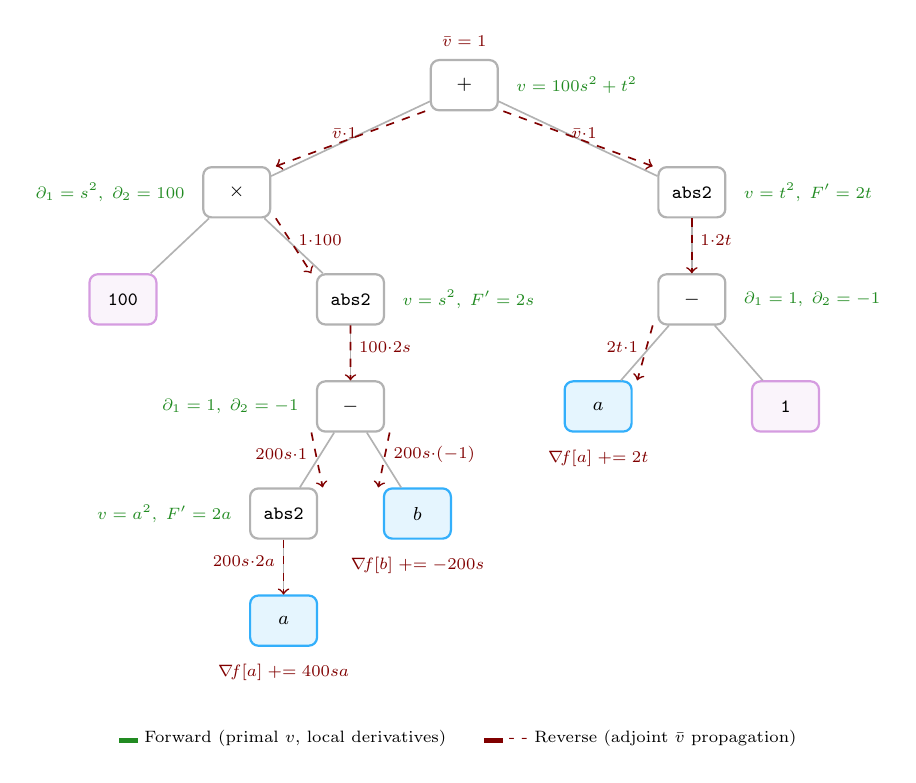
\begin{tikzpicture}[
  scale=0.85, transform shape,
  nd/.style={rectangle, rounded corners=3pt, draw=gray!60, thick, fill=white,
    minimum height=7.5mm, minimum width=10mm, inner sep=2pt, font=\footnotesize\ttfamily},
  ndvar/.style={nd, draw=j1!80, fill=j1!10},
  ndconst/.style={nd, draw=j4!70, fill=j4!8},
  fwd/.style={font=\scriptsize, text=ForestGreen},
  rev/.style={font=\scriptsize, text=Maroon},
  edge from parent/.style={draw, gray!60, semithick},
  level 1/.style={sibling distance=68mm, level distance=16mm},
  level 2/.style={sibling distance=34mm, level distance=16mm},
  level 3/.style={sibling distance=28mm, level distance=16mm},
  level 4/.style={sibling distance=20mm, level distance=16mm},
]

% --- Single tree with both annotations ---
\node[nd] (plus) {$+$}
  child { node[nd] (times) {$\times$}
    child { node[ndconst] (c100) {100} }
    child { node[nd] (sq1) {abs2}
      child { node[nd] (sub1) {$-$}
        child { node[nd] (sq2) {abs2}
          child { node[ndvar] (va1) {$a$} }
        }
        child { node[ndvar] (vb) {$b$} }
      }
    }
  }
  child { node[nd] (sq3) {abs2}
    child { node[nd] (sub2) {$-$}
      child { node[ndvar] (va2) {$a$} }
      child { node[ndconst] (c1) {1} }
    }
  };

% --- Forward pass annotations (green, right side) ---
\node[fwd, right=4pt of plus, anchor=west] {$v = 100s^2 + t^2$};
\node[fwd, left=4pt of times, anchor=east] {$\partial_1 = s^2,\; \partial_2 = 100$};
\node[fwd, right=4pt of sq1, anchor=west] {$v = s^2,\; F' = 2s$};
\node[fwd, left=4pt of sub1, anchor=east] {$\partial_1 = 1,\; \partial_2 = {-}1$};
\node[fwd, left=4pt of sq2, anchor=east] {$v = a^2,\; F' = 2a$};
\node[fwd, right=4pt of sq3, anchor=west] {$v = t^2,\; F' = 2t$};
\node[fwd, right=4pt of sub2, anchor=west] {$\partial_1 = 1,\; \partial_2 = {-}1$};

% --- Reverse pass annotations (maroon, arrows with edge labels) ---
\node[rev, above=2pt of plus, anchor=south] {$\bar{v} = 1$};

% Adjoint propagation arrows (dashed, maroon)
\draw[->, Maroon, semithick, dashed] ([xshift=-2pt]plus.south west) --
  node[left, rev, pos=0.4] {$\bar{v}{\cdot}1$} ([xshift=2pt]times.north east);
\draw[->, Maroon, semithick, dashed] ([xshift=2pt]plus.south east) --
  node[right, rev, pos=0.4] {$\bar{v}{\cdot}1$} ([xshift=-2pt]sq3.north west);

\draw[->, Maroon, semithick, dashed] ([xshift=2pt]times.south east) --
  node[right, rev, pos=0.4] {$1{\cdot}100$} ([xshift=-2pt]sq1.north west);

\draw[->, Maroon, semithick, dashed] (sq1.south) --
  node[right, rev, pos=0.4] {$100{\cdot}2s$} (sub1.north);

\draw[->, Maroon, semithick, dashed] ([xshift=-2pt]sub1.south west) --
  node[left, rev, pos=0.4] {$200s{\cdot}1$} ([xshift=2pt]sq2.north east);
\draw[->, Maroon, semithick, dashed] ([xshift=2pt]sub1.south east) --
  node[right, rev, pos=0.4] {$200s{\cdot}({-}1)$} ([xshift=-2pt]vb.north west);

\draw[->, Maroon, semithick, dashed] (sq2.south) --
  node[left, rev, pos=0.4] {$200s{\cdot}2a$} (va1.north);

\draw[->, Maroon, semithick, dashed] (sq3.south) --
  node[right, rev, pos=0.4] {$1{\cdot}2t$} (sub2.north);
\draw[->, Maroon, semithick, dashed] ([xshift=-2pt]sub2.south west) --
  node[left, rev, pos=0.4] {$2t{\cdot}1$} ([xshift=2pt]va2.north east);

% --- Gradient results at leaves ---
\node[rev, font=\scriptsize\bfseries, below=4pt of va1, anchor=north] {$\nabla\!f[a] \mathrel{+}= 400sa$};
\node[rev, font=\scriptsize\bfseries, below=4pt of vb, anchor=north] {$\nabla\!f[b] \mathrel{+}= {-}200s$};
\node[rev, font=\scriptsize\bfseries, below=4pt of va2, anchor=north] {$\nabla\!f[a] \mathrel{+}= 2t$};

% --- Legend ---
\node[anchor=north, font=\scriptsize] at ([yshift=-5mm]current bounding box.south) {
  \textcolor{ForestGreen}{\rule{8pt}{2pt}}~Forward (primal $v$, local derivatives)\qquad
  \textcolor{Maroon}{\rule{8pt}{2pt}}~\textcolor{Maroon}{- -}~Reverse (adjoint $\bar{v}$ propagation)
};
\end{tikzpicture}
\caption{First-order reverse-mode AD on the Rosenbrock pattern $f_i = 100(a^2 - b)^2 + (a - 1)^2$ with $a = x_{i-1}$, $b = x_i$, $s = a^2 - b$, $t = a - 1$ (same tree as Figure~\ref{fig:tree}, with \texttt{Var} index subtrees collapsed). \textcolor{ForestGreen}{Green} labels show the forward pass: each node stores its primal value $v$ and local derivatives $F'$ or $\partial_1, \partial_2$. \textcolor{Maroon}{Maroon} dashed arrows show the reverse pass: the adjoint $\bar{v}=1$ at the root is multiplied by each node's local derivative and propagated to its children. At the leaves, accumulated adjoints give the gradient: $\partial f_i/\partial x_{i-1} = 400sa + 2t$ and $\partial f_i/\partial x_i = -200s$.}
\label{fig:ad}
\end{figure}

For the sparse Jacobian callback \texttt{jac\_coord!}, ExaModels.jl uses a sparse variant \texttt{grpass} that replaces the dense accumulation $\nabla f[i] \mathrel{+}= \bar{v}$ with a compressed write $v[\text{offset} + \texttt{comp}(\text{cnt})] \mathrel{+}= \bar{v}$, where \texttt{comp} is a \texttt{Compressor} that maps the sequential leaf counter to the correct position in the COO value array. The sparsity structure and the \texttt{Compressor} are precomputed at model-construction time (Section~\ref{sec:ad:sparsity}).

\subsection{Second-Order Derivatives}
\label{sec:ad:second}

The Hessian of the Lagrangian requires second-order derivatives. ExaModels.jl extends the two-phase approach by constructing a \emph{second-adjoint tree} and performing a more elaborate reverse pass.

\paragraph{Forward pass.}
The expression tree is evaluated with \texttt{SecondAdjointNodeSource(x)}, producing a second-adjoint tree where each node stores the primal value, first derivatives, \emph{and} second derivatives:
\begin{itemize}
  \item \texttt{SecondAdjointNode1\{F\}}: stores $v = F(u)$, $y = F'(u)$, and $h = F''(u)$.
  \item \texttt{SecondAdjointNode2\{F\}}: stores $v$, $y_1 = \partial_1 F$, $y_2 = \partial_2 F$, $h_{11} = \partial_{11} F$, $h_{12} = \partial_{12} F$, $h_{22} = \partial_{22} F$.
\end{itemize}
The second derivatives $F''$, $\partial_{11} F$, etc.\ are supplied by \texttt{ddf} and \texttt{ddf11}, \texttt{ddf12}, \texttt{ddf22} from the function registration macros.

\paragraph{Reverse pass.}
The reverse pass propagates a pair $(\bar{v}, \bar{v}_2)$---the first and second adjoints---from root to leaves. Two mutually recursive functions implement this:
\begin{itemize}
  \item \texttt{hrpass} (diagonal pass): at a \texttt{SecondAdjointNode1\{F\}} with derivatives $y = F'$ and $h = F''$, it propagates to the child:
  \[
    \bar{v}_{\text{child}} = \bar{v} \cdot y, \qquad
    \bar{v}_{2,\text{child}} = \bar{v}_2 \cdot y^2 + \bar{v} \cdot h.
  \]
  At a \texttt{SecondAdjointNode2\{F\}}, it propagates to each child analogously and calls \texttt{hdrpass} for the cross term.
  \item \texttt{hdrpass} (cross-derivative pass): traverses \emph{two} subtrees simultaneously, computing the mixed partial contributions $\bar{v}_2 \cdot y_1 y_2 + \bar{v} \cdot h_{12}$ between subtree pairs. At the leaves, when both subtrees reach \texttt{SecondAdjointNodeVar} nodes with indices $i$ and $j$, the Hessian entry $H[i,j]$ is accumulated.
\end{itemize}
At a \texttt{SecondAdjointNodeVar} leaf with index $i$, \texttt{hrpass} accumulates the diagonal Hessian entry $H[i,i] \mathrel{+}= \bar{v}_2$.

\paragraph{Linear node optimization.}
Many expression trees contain long chains of affine operations ($+$, $-$, multiplication by a constant) whose second derivatives are identically zero. ExaModels.jl exploits this with \texttt{hrpass0}, a specialized entry point that dispatches on the function type: for affine \texttt{SecondAdjointNode1} nodes (e.g., \texttt{FirstFixed\{typeof(*)\}}, \texttt{SecondFixed\{typeof(+)\}}), the $h$ term is known to be zero at compile time, and the recursion propagates only $(\bar{v} \cdot y,\; \bar{v}_2 \cdot y^2)$ without computing the $\bar{v} \cdot h$ contribution. This eliminates unnecessary multiplications and additions in the hot inner loop, particularly for the common case of weighted sums of nonlinear terms.

\paragraph{Remark.}
The forward--reverse AD procedure described above is standard in the AD literature. What distinguishes ExaModels.jl is that these passes are applied to the \emph{parameterized} expression tree from Section~\ref{sec:graph}: the same compiled AD code is executed across all data points of a pattern in an embarrassingly parallel fashion. For a pattern with $I$ data points, the forward and reverse passes are independent across $i \in [I]$---each invocation reads different variable indices (via \texttt{DataIndexed}) and writes to different sparse output positions (via the \texttt{Compressor} offsets). This data-parallel structure maps directly to the SIMD abstraction of Section~\ref{sec:modeling:simd} and is the basis for GPU acceleration (Section~\ref{sec:gpu}).

\subsection{Sparsity Detection Without Coloring}
\label{sec:ad:sparsity}

A major advantage of the SIMD abstraction is that the sparsity structure of each pattern can be determined \emph{a priori} at model-construction time, eliminating the need for graph coloring---a step that is typically required by conventional AMSs to compress sparse Jacobian and Hessian evaluations.

\paragraph{Probe evaluation.}
For each pattern, ExaModels.jl performs a single probe evaluation of the expression tree using sentinel arguments. The primal vector $x$ is replaced by a \texttt{NaNSource} (returning \texttt{NaN} for any index), and the data point $i$ is replaced by an \texttt{Identity} sentinel. Under these sentinels, the \texttt{DataIndexed} nodes evaluate to \texttt{NaN} (since no real data is available), while the \texttt{Var} nodes record which symbolic variable indices are visited. The AD reverse passes (\texttt{grpass} for first-order, \texttt{hrpass0} for second-order) are then executed on this probed tree with the \texttt{Compressor} argument set to \texttt{nothing}, triggering a special dispatch that \emph{collects} the raw sequence of variable index visits rather than accumulating numeric values.

\paragraph{Compressor.}
The raw sequence collected by the probe may contain duplicate entries (e.g., if $x_i$ appears multiple times in the expression). The \texttt{Compressor} is a mapping from the raw sequence position to the unique nonzero index:
\begin{enumerate}
  \item Compute the list of unique variable indices (for the Jacobian) or unique $(i,j)$ pairs (for the Hessian) from the raw probe output.
  \item Build a mapping tuple: for each entry in the raw sequence, record which unique index it corresponds to.
  \item Store this mapping as a compile-time tuple \texttt{Compressor\{I\}}, where \texttt{I} is an \texttt{NTuple\{N,Int\}}.
\end{enumerate}
Because the mapping is stored as a type parameter (an \texttt{NTuple}), looking up \texttt{comp(cnt)} is a constant-time, inlined operation with no runtime allocation.

\paragraph{Offset computation.}
During the AD reverse pass at evaluation time, a running counter \texttt{cnt} is incremented each time a leaf node is reached. The sparse output position is computed as $\text{offset} + \texttt{comp}(\texttt{cnt})$, where the offset locates this pattern's block within the global COO array, and \texttt{comp} maps the counter to the correct position among the pattern's unique nonzeros. The offset advances by $\text{o1step}$ (for the Jacobian) or $\text{o2step}$ (for the Hessian) for each data point, so data point $k$ writes to positions $[\text{o1} + (k{-}1) \cdot \text{o1step} + 1,\, \ldots,\, \text{o1} + k \cdot \text{o1step}]$. Because each data point has the same number of unique nonzeros (determined by the pattern, not the data), the offsets are perfectly regular---no dynamic bookkeeping is needed.

\paragraph{Why coloring is unnecessary.}
In conventional AMSs, the Jacobian and Hessian sparsity patterns are determined for the \emph{entire} monolithic expression graph, and graph coloring is used to identify groups of structurally independent columns that can be evaluated simultaneously. This coloring step is itself expensive and must be performed before derivatives can be computed. In ExaModels.jl, the SIMD structure makes coloring unnecessary: each pattern touches only $O(1)$ variables (determined by the expression tree depth, not the problem size), so the per-pattern sparsity is small and fixed. The \texttt{Compressor} precomputes the exact nonzero positions within each pattern, and the regular stride across data points means the global COO structure is assembled by simple concatenation of pattern blocks. The entire sparsity analysis is performed once per pattern at model-construction time and has negligible cost relative to the solve.

\paragraph{Partially compressed COO format.}
The resulting Jacobian and Hessian are stored in a \emph{partially compressed} coordinate format. Within each pattern, the \texttt{Compressor} identifies and merges duplicate nonzero entries that arise from the same expression tree (e.g., when a variable appears multiple times in the same expression). However, we deliberately do \emph{not} compress across different patterns or across different data points of the same pattern. This means that if two patterns contribute to the same $(i,j)$ entry of the Hessian, they write to separate positions in the COO array, and the solver's sparse matrix assembly performs the final summation. This design choice has two key benefits: (i) it ensures that different patterns---and different data points within a pattern---never write to the same memory location, eliminating write conflicts and enabling lock-free parallel evaluation; and (ii) it allows the same compiled kernel to be executed identically for every data point in a pattern, with only the offset advancing by a fixed stride. The trade-off is a moderately larger COO array (proportional to the total number of pattern$\times$data-point contributions rather than the number of unique structural nonzeros), but this is acceptable because the evaluation cost is dominated by the kernel arithmetic, not the array storage.

\section{GPU Acceleration and Implementation}
\label{sec:gpu}

The SIMD abstraction of Section~\ref{sec:modeling:simd} maps naturally to GPU execution: each computational pattern becomes a GPU kernel, and each data point becomes a thread. Because all threads within a pattern execute the same compiled expression tree on different data indices, there is no thread divergence---every thread follows the same control flow, which is ideal for GPU hardware. This section describes how ExaModels.jl implements this mapping, using KernelAbstractions.jl~\cite{churavyKernelAbstractionsjl2025} for backend-agnostic GPU kernels, and discusses the key implementation choices that affect performance on both CPU and GPU.

\subsection{SIMDFunction: the Compiled Pattern}
\label{sec:gpu:simdfunction}

The central compilation artifact in ExaModels.jl is the \texttt{SIMDFunction}, which bundles everything needed to evaluate a pattern and its derivatives:
\begin{lstlisting}
struct SIMDFunction{F,C1,C2}
    f::F          # parameterized expression tree
    comp1::C1     # Compressor for Jacobian sparsity
    comp2::C2     # Compressor for Hessian sparsity
    o0::Int       # offset into constraint/objective vector
    o1::Int       # offset into Jacobian COO array
    o2::Int       # offset into Hessian COO array
    o1step::Int   # stride per data point (Jacobian)
    o2step::Int   # stride per data point (Hessian)
end
\end{lstlisting}
Here, \texttt{f} is the parameterized expression tree from Section~\ref{sec:graph}, \texttt{comp1} and \texttt{comp2} are the \texttt{Compressor} mappings from Section~\ref{sec:ad:sparsity}, and the six integer fields locate this pattern's output within the global COO arrays. Each \texttt{Objective} and \texttt{Constraint} in the model wraps a \texttt{SIMDFunction} together with an iterator \texttt{itr} over data points.

To make the idea concrete, consider the Rosenbrock pattern $100(x_{i-1}^2 - x_i)^2 + (x_{i-1} - 1)^2$ from Section~\ref{sec:graph}. This pattern touches two variables per data point, so its Jacobian has 2 unique entries per data point (\texttt{o1step} $= 2$) and its Hessian has 3 unique entries (\texttt{o2step} $= 3$: the two diagonal entries and one off-diagonal). The \texttt{Compressor} tuples encode the mapping from the AD leaf-visit order to these unique entries, and the offsets \texttt{o1}, \texttt{o2} locate the block within the global arrays.

\subsection{CPU vs.\ GPU Evaluation}
\label{sec:gpu:cpugpu}

On the CPU, each callback iterates over patterns using a tuple-recursive dispatch, and within each pattern, a \texttt{@simd for} loop iterates over data points sequentially:
\begin{lstlisting}
# CPU constraint evaluation (simplified)
@simd for i in eachindex(con.itr)
    @inbounds g[offset0(con, i)] += con.f(con.itr[i], x, $\theta$)
end
\end{lstlisting}
The call \texttt{con.f(con.itr[i], x, $\theta$)} evaluates the parameterized expression tree for data point $i$; the SIMD annotation enables the compiler to vectorize across data points using CPU SIMD instructions.

On the GPU, the same loop body becomes the kernel function, and data points are mapped to GPU threads. The following listing shows the actual KernelAbstractions.jl kernel used for constraint evaluation in \texttt{ExaModelsKernelAbstractions.jl}:
\begin{lstlisting}
@kernel function kerf(y, @Const(f), @Const(itr),
                      @Const(x), @Const($\theta$))
    I = @index(Global)
    @inbounds y[offset0(f, itr, I)] = f(itr[I], x, $\theta$)
end
\end{lstlisting}
Each GPU thread computes exactly one data point: \texttt{@index(Global)} provides the thread's global index $I$, and the expression tree \texttt{f} is evaluated at data point \texttt{itr[I]} to produce the constraint value. The kernel is launched with \texttt{ndrange = length(itr)}, assigning one thread per data point. Because \texttt{f} is a fully typed, compile-time-specialized expression tree (Section~\ref{sec:graph:type}), the kernel contains no dynamic dispatch---a requirement for GPU compilation.

The same pattern applies to derivative kernels. The sparse gradient kernel launches one thread per data point and executes the full forward--reverse AD pass (Section~\ref{sec:ad}) within that thread:
\begin{lstlisting}
@kernel function kerg_sparse(y, @Const(f), @Const(itr),
        @Const(x), @Const($\theta$), @Const(adj), ...)
    I = @index(Global)
    @inbounds grpass(
        f(itr[I], AdjointNodeSource(x), $\theta$),
        f.comp1, y, offset1(f, I), 0, adj)
end
\end{lstlisting}
Each thread independently builds the adjoint tree for its data point, traverses it in reverse, and writes gradient entries to the sparse output array at positions determined by the \texttt{Compressor} and offsets. The Jacobian and Hessian kernels follow the same structure, calling \texttt{jrpass} and \texttt{hrpass0} respectively.

KernelAbstractions.jl~\cite{churavyKernelAbstractionsjl2025} provides the backend abstraction layer. All kernels are written once using the \texttt{@kernel} macro and run on any supported backend: CUDA.jl (NVIDIA), AMDGPU.jl (AMD), oneAPI.jl (Intel), Metal.jl (Apple), and the \texttt{CPU()} backend for multithreaded execution on the host. The user selects the backend at model-construction time via \texttt{ExaCore(; backend = CUDABackend())}, and no model code changes are needed.

\subsection{Implementation Details}
\label{sec:gpu:impl}

Several implementation choices are worth noting, as they affect both correctness and performance.

\paragraph{Sparse evaluation without compression.}
For Jacobian and Hessian evaluation, each data point in a pattern writes to its own contiguous block of the COO value array (Section~\ref{sec:ad:sparsity}). Because different data points write to disjoint positions, no atomics or synchronization are needed---all writes are conflict-free. This is a direct consequence of the SIMD structure: within a pattern, data point $k$ writes to positions starting at $\texttt{o1} + (k{-}1) \cdot \texttt{o1step}$. ExaModels.jl therefore stores Jacobian and Hessian entries in COO format natively and does \emph{not} convert to CSC (Compressed Sparse Column) format. This avoids the compression step---which would require sorting and merging entries---and is well suited for solvers like MadNLP.jl~\cite{shinMadNLPjl2025} that accept COO input directly.

\paragraph{Objective: buffer and reduce.}
The objective callback evaluates $f(x) = \sum_\ell \sum_{i=1}^{I_\ell} \tilde{f}^{(\ell)}(p_i, x, \theta)$ (Equation~\ref{eq:simdfunction}). On the CPU, this is computed by direct scalar accumulation in a loop. On the GPU, each thread writes its pattern evaluation into a buffer of length $\sum_\ell I_\ell$, and the final objective value is obtained by a parallel reduction (\texttt{sum}). This two-phase approach---evaluate into buffer, then reduce---avoids atomic additions to a single scalar.

\paragraph{Gradient: sparse evaluation then compression.}
On the CPU, the gradient is computed by the dense reverse pass (\texttt{drpass}, Section~\ref{sec:ad:first}), which directly accumulates $\nabla f[i] \mathrel{+}= \bar{v}$ into the dense gradient vector. On the GPU, the sparse reverse pass (\texttt{grpass}) is used instead: each thread writes gradient contributions into a sparse buffer indexed by \texttt{(variable\_index, position)}, and a subsequent \texttt{compress\_to\_dense} kernel reduces the sparse buffer into the dense gradient vector. This two-phase approach is necessary because multiple threads (from different patterns) may contribute to the same gradient entry, and atomic additions to a dense vector would cause contention:
\begin{lstlisting}
@kernel function compress_to_dense(y, @Const(y0),
        @Const(ptr), @Const(sparsity))
    I = @index(Global)
    @inbounds for j = ptr[I]:(ptr[I+1]-1)
        (k, l) = sparsity[j]
        y[k] += y0[l]
    end
end
\end{lstlisting}
The \texttt{ptr} array partitions the sparse buffer entries by target variable, so each thread in the compression kernel handles a distinct set of target indices without conflicts.

\paragraph{Data-level parallelism only.}
ExaModels.jl parallelizes at the data-point level: each thread executes the full forward--reverse AD pass for one data point of one pattern. The expression tree itself is \emph{not} decomposed or parallelized internally---there is no intra-tree parallelism. This design keeps the kernel simple and avoids the synchronization overhead that would arise from parallelizing the tree traversal. For typical NLP patterns, the expression trees are small (tens of nodes), so the parallelism from thousands of data points is more than sufficient to saturate GPU hardware. The result is high occupancy with minimal kernel launch overhead: one kernel launch per pattern per callback.


\section{Type Stability and Ahead-of-Time Compilation}
\label{sec:aot}

A Julia function is \emph{type-stable} if the compiler can infer the concrete type of every variable and return value from the types of the arguments alone, with no runtime dispatch. Type stability is not merely a performance optimization: GPU kernels \emph{require} it (dynamic dispatch is not supported on GPU hardware), and Julia's ahead-of-time (AOT) compiler \texttt{juliac --trim=safe} relies on it to produce standalone binaries with unused code eliminated. This section explains how ExaModels.jl achieves full type stability through its design, and how this enables AOT compilation of complete optimization applications.

\subsection{Immutable ExaCore and Reconstruction}
\label{sec:aot:exacore}

The central design choice that enables type stability is that \texttt{ExaCore} is an \emph{immutable} struct (not \texttt{mutable struct}). Each call to \texttt{@add\_var}, \texttt{@add\_obj}, or \texttt{@add\_con} creates a \emph{new} \texttt{ExaCore} with a different concrete type:
\begin{lstlisting}
c = ExaCore()                  # ExaCore{..., Tuple{}, Tuple{}}
c, x = @add_var(c, x, N)      # ExaCore{..., Tuple{Variable}, Tuple{}}
@add_obj(c, 100(x[i]^2 - x[i+1])^2 + (x[i] - 1)^2 for i = 1:N-1)
#              ExaCore{..., Tuple{Variable}, Tuple{Objective{...}}}
\end{lstlisting}
Because the tuple of objectives and constraints grows by prepending, each step produces an \texttt{ExaCore} whose type encodes the \emph{exact} set of patterns added so far. The Julia compiler sees these as distinct concrete types and generates specialized code for each construction step. When \texttt{ExaModel(c)} is called, the final \texttt{ExaCore} type fully determines the structure of the compiled model, including all expression trees, \texttt{Compressor} tuples, and offset computations.

This is a deliberate contrast with the approach taken by JuMP~\cite{lubinJuMP10Recent2023} and similar AMSs, where the model object is a mutable container that accumulates variables, constraints, and objectives behind a single stable type. In JuMP, each \texttt{@variable}, \texttt{@constraint}, and \texttt{@objective} mutates internal dictionaries within the same \texttt{Model} object:
\begin{lstlisting}
m = Model(Ipopt.Optimizer)
@variable(m, x[1:N])                  # mutates m
@constraint(m, [i=1:N-2], g(x,i)==0)  # mutates m
@objective(m, Min, sum(f(x,i) for i=1:N-1))  # mutates m
\end{lstlisting}
This API is natural and ergonomic, but the model's concrete type does not change across these calls---all structure is hidden in runtime data structures. As a result, the derivative evaluation code necessarily involves dynamic dispatch over the stored expression types, precluding the kind of compile-time specialization described in Sections~\ref{sec:graph:type} and~\ref{sec:gpu:cpugpu}.

The ExaModels.jl macro syntax (\texttt{@add\_var}, \texttt{@add\_obj}, \texttt{@add\_con}) is designed to \emph{look} like the JuMP convention while achieving the opposite effect: each macro call reassigns the variable \texttt{c} to a new, differently-typed \texttt{ExaCore}, so that the compiler can track the growing model structure statically. The user writes:
\begin{lstlisting}
c = ExaCore(concrete = Val(true))
c, x = @add_var(c, x, N; start = (x0(i) for i=1:N))
@add_con(c, g(x, i) for i = 1:N-2)
@add_obj(c, f(x, i) for i = 1:N-1)
m = ExaModel(c)
\end{lstlisting}
which reads like a conventional modeling script, but each line produces a new concrete type that the compiler can fully specialize.

\subsection{Ahead-of-Time Compilation}
\label{sec:aot:juliac}

Because all ExaModels.jl code paths are type-stable, the entire model construction and solve pipeline is compatible with Julia's AOT compiler \texttt{juliac --trim=safe}, which produces a standalone binary or shared library with no Julia runtime dependency. Combined with NLPModelsIpoptLite.jl---a lightweight, AOT-compatible wrapper around the Ipopt C library---a complete optimization application can be packaged as a single executable:
\begin{lstlisting}
# RosenbockApp.jl --- compiles to a binary
module RosenbrockApp
using ExaModels, NLPModelsIpoptLite
function (@main)(ARGS)
    N = parse(Int, ARGS[1])
    c = ExaCore(concrete = Val(true))
    c, x = @add_var(c, x, N; start = (mod(i,2)==1 ? -1.2 : 1.0 for i=1:N))
    @add_obj(c, 100(x[i]^2 - x[i+1])^2 + (x[i] - 1)^2 for i = 1:N-1)
    m = ExaModel(c)
    result = ipopt(m; print_level = 5)
    return result.status == 0 ? 0 : 1
end
end
\end{lstlisting}
Running \texttt{juliac --trim=safe --output-exe rosenbrock RosenbrockApp.jl} produces a standalone binary that solves the Rosenbrock problem for any $N$ specified at the command line, with no JIT compilation latency. As of this writing, AOT compilation is supported for CPU backends only; GPU backends still require Julia's JIT runtime for kernel compilation.

\subsection{Generic Numeric Precision}
\label{sec:aot:precision}

Julia's multiple dispatch and JIT compilation make the entire ExaModels.jl pipeline---expression tree construction, AD evaluation, and solver callbacks---generic over the floating-point type. All internal code operates on the abstract type \texttt{T <: AbstractFloat}, and the compiler specializes automatically:
\begin{lstlisting}
c32 = ExaCore(Float32)  # all arrays use Float32
c64 = ExaCore(Float64)  # all arrays use Float64
\end{lstlisting}
This extends to user-defined numeric types. For example, using DoubleFloats.jl for quadruple precision requires no code changes beyond specifying the type at \texttt{ExaCore} construction. The \texttt{Constant\{T\}} type parameter (Section~\ref{sec:graph:constants}) ensures that compile-time constants are converted to the appropriate precision via \texttt{replace\_T}, so no mixed-precision artifacts arise.

This flexibility is particularly valuable for GPU computation, where \texttt{Float32} arithmetic is significantly faster than \texttt{Float64} on consumer GPUs, and for applications requiring extended precision (e.g., sensitivity analysis near degeneracy).

\subsection{Best Practices for Model Library Developers}
\label{sec:aot:bestpractices}

Developers building reusable model libraries on top of ExaModels.jl (e.g., \texttt{ExaModelsPower.jl}, \texttt{COPSBenchmark.jl}) should follow three guidelines to ensure their models are maximally portable and efficient:
\begin{enumerate}
  \item \textbf{Do not hardcode the numeric type.} Accept the floating-point type as a parameter and pass it to \texttt{ExaCore(T; ...)}. This allows users to switch between \texttt{Float64}, \texttt{Float32}, and extended-precision types without modifying the model code.
  \item \textbf{Accept the backend as a parameter.} The model constructor should take a \texttt{backend} keyword (defaulting to \texttt{nothing} for CPU) and pass it to \texttt{ExaCore(T; backend = backend)}. This enables users to run the same model on any GPU backend without modifying the library.
  \item \textbf{Ensure type stability.} Use \texttt{concrete = Val(true)} and avoid type-unstable patterns (storing models in untyped containers, using global mutable state). Type-stable model code is required for AOT compilation and also yields better JIT performance. While this third guideline is optional for correctness, it is strongly recommended for production use.
\end{enumerate}
For example, a portable model constructor follows this pattern:
\begin{lstlisting}
function my_model(data; T = Float64, backend = nothing)
    core = ExaCore(T; backend = backend, concrete = Val(true))
    @add_var(core, x, length(data))
    @add_obj(core, f(x, data[i]) for i in eachindex(data))
    return ExaModel(core)
end
\end{lstlisting}

\section{Solver Interface}
\label{sec:interface}

ExaModels.jl connects to NLP solvers through the NLPModels.jl callback interface\footnote{\url{https://github.com/JuliaSmoothOptimizers/NLPModels.jl}}, which was introduced in Section~\ref{sec:modeling:nlp}. An \texttt{ExaModel} is a concrete subtype of \texttt{AbstractNLPModel} and implements the five callbacks \eqref{eq:callbacks} using the AD machinery of Section~\ref{sec:ad}. The solver never sees the expression trees or the SIMD decomposition---it interacts with the model exclusively through the callback API, receiving objective values, gradient vectors, constraint vectors, and sparse Jacobian/Hessian entries in COO format.

This callback-based interface is fundamentally different from the approach taken by MathOptInterface (MOI)~\cite{lubinJuMP10Recent2023}, which transmits the problem to the solver as an algebraic expression tree or a structured matrix representation. MOI is well suited for LP, QP, and MIP solvers that exploit problem structure at the formulation level. For nonlinear interior-point solvers---which require repeated derivative evaluations at changing iterates---the callback-based approach is the natural fit: the AMS retains control over the derivative computation, and the solver simply requests numerical values.

The NLPModels.jl interface gives ExaModels.jl access to the broad solver ecosystem of the JuliaSmoothOptimizers (JSO) organization. Any solver that accepts an \texttt{AbstractNLPModel} works out of the box. The following general-purpose NLP solvers are currently available:
\begin{itemize}
  \item \textbf{Ipopt}~\cite{wachterImplementationInteriorpointFilter2006} (via NLPModelsIpopt.jl) --- interior-point filter line-search method,
  \item \textbf{KNITRO}~\cite{byrdKnitroIntegratedPackage2006} (via NLPModelsKnitro.jl) --- commercial interior-point / active-set solver,
  \item \textbf{MadNLP.jl}~\cite{shinMadNLPjl2025} --- Julia-native interior-point solver with GPU support, enabling a fully GPU-resident optimization pipeline when paired with ExaModels.jl,
  \item \textbf{Uno}\footnote{\url{https://github.com/cvanaret/Uno}} (via Uno.jl) --- modular SQP and barrier solver,
  \item \textbf{Percival.jl} --- augmented Lagrangian method for equality-constrained problems,
  \item \textbf{DCISolver.jl} --- dynamic control of infeasibility method,
  \item \textbf{FletcherPenaltySolver.jl} --- Fletcher's smooth exact penalty method.
\end{itemize}
Additionally, the JSO ecosystem provides unconstrained and bound-constrained solvers (JSOSolvers.jl, AdaptiveRegularization.jl) and specialized solvers for least-squares problems (CaNNOLeS.jl) and linear/quadratic programs (RipQP.jl), all of which accept \texttt{AbstractNLPModel} inputs. The ecosystem also includes utility packages such as NLPModelsModifiers.jl, which provides model transformations (e.g., slack reformulations, feasibility problems, and regularization wrappers) that can be composed with any \texttt{AbstractNLPModel}---including \texttt{ExaModel}---without modifying the underlying model code. No glue code or solver-specific adaptation is needed: the user constructs an \texttt{ExaModel} and passes it directly to any of these solvers or utilities.

\section{Extensions}
\label{sec:extensions}

The SIMD formulation \eqref{eq:simd} captures a single deterministic NLP. Many applications require solving families of related NLPs---varying parameters, coupling through shared design variables, or solving independent instances simultaneously. ExaModels.jl supports these through three orthogonal extensions that can be \emph{combined simultaneously}: parameterized problems, two-stage stochastic programs, and batch models.

\subsection{Unified Formulation}
\label{sec:extensions:formulation}

The most general formulation supported by ExaModels.jl is a \emph{batched two-stage parametric} NLP. Given $B$ independent batch instances and $S$ scenarios per instance, the problem is:
\begin{equation}\label{eq:extensions}
\begin{aligned}
  \min_{d_b,\, v_{b,1}, \ldots, v_{b,S}}\quad & f_0(d_b;\, \theta_{b}) + \sum_{s=1}^{S} f_s(d_b, v_{b,s};\, \theta_{b,s}), \quad b \in [B], \\
  \st\quad & g_0(d_b;\, \theta_{b}) \in \mathcal{C}_0, \quad b \in [B], \\
           & g_s(d_b, v_{b,s};\, \theta_{b,s}) \in \mathcal{C}_s, \quad s \in [S],\; b \in [B],
\end{aligned}
\end{equation}
where $d_b$ are the first-stage (design) variables, $v_{b,s}$ are the second-stage (recourse) variables for scenario~$s$ of instance~$b$, $\theta_{b}$ and $\theta_{b,s}$ are parameters (not optimized over), and each $f_s$, $g_s$ has the SIMD structure of \eqref{eq:simd}. The three extensions correspond to the three dimensions of this formulation:
\begin{itemize}
  \item \textbf{Parameters} ($\theta$): the patterns depend on $\theta$, which can be updated via \texttt{set\_value!} without recompiling the model.
  \item \textbf{Two-stage structure} ($S > 1$): design variables $d_b$ are shared across scenarios; recourse variables $v_{b,s}$ and constraints $g_s$ are replicated per scenario.
  \item \textbf{Batch structure} ($B > 1$): independent instances share the same compiled expression trees but differ in parameter values $\theta_{b,s}$.
\end{itemize}
Setting $S = 1$ and $B = 1$ recovers the base formulation \eqref{eq:simd}. Setting $B = 1$ gives a standard two-stage stochastic program. Setting $S = 1$ with no shared variables gives a batch model. All three can be active simultaneously.

A critical design principle is that all scenarios and batch instances share the \emph{same compiled expression patterns}. The \texttt{SIMDFunction}s, \texttt{Compressor} maps, and sparsity structures are built once and reused across every scenario and instance. The only quantities that vary across scenarios or instances are \emph{numerical data}: parameter values~$\theta$, variable bounds ($x^\flat$, $x^\sharp$), constraint bounds ($g^\flat$, $g^\sharp$), and initial points ($x_0$, $y_0$). This is what makes the extensions efficient---no model recompilation is needed when changing these numerical quantities. Accordingly, ExaModels.jl provides per-scenario and per-instance getters and setters:
\begin{itemize}
  \item \texttt{set\_value!(m, p, vals, scen)} --- update parameter block \texttt{p} for scenario \texttt{scen}.
  \item \texttt{set\_start!(m, x, vals, scen)}, \texttt{set\_lvar!(m, x, vals, scen)}, etc.\ --- update initial points and bounds for scenario \texttt{scen} (two-stage) or instance \texttt{scen} (batch).
  \item \texttt{get\_value(m, p, scen)}, \texttt{get\_start(m, x, scen)}, etc.\ --- the corresponding queries.
\end{itemize}
These accessors modify only the underlying numerical arrays ($\theta$, $x_0$, bounds) without touching the compiled model structure.

\subsection{Syntax: \texttt{EachScenario()} and \texttt{BatchExaCore}}
\label{sec:extensions:syntax}

ExaModels.jl provides two core constructors and one marker type to express the formulation \eqref{eq:extensions}:
\begin{itemize}
  \item \texttt{TwoStageExaCore(nscen)} creates a core for \texttt{nscen} scenarios. The marker type \texttt{EachScenario()} distinguishes first-stage from second-stage declarations: \texttt{@add\_var(c, x, n)} adds design variables shared across all scenarios, while \texttt{@add\_var(c, EachScenario(), v, n)} adds recourse variables replicated per scenario. The same marker works for \texttt{@add\_par}, \texttt{@add\_obj}, and \texttt{@add\_con}.
  \item \texttt{BatchExaCore(nbatch)} creates a core for \texttt{nbatch} independent instances. All declarations are implicitly replicated across instances; internally, the storage switches from vectors to matrices of size $n \times B$.
\end{itemize}
These can be combined: \texttt{TwoStageExaCore(nscen; nbatch = Val(B))} creates a batched two-stage core. The following example illustrates all three extensions simultaneously:
\begin{lstlisting}
B, S = 4, 10                                # 4 instances, 10 scenarios each
core = TwoStageExaCore(S; nbatch = Val(B))
core, d = @add_var(core, d, n_d)                  # design (shared across scenarios)
core, v = @add_var(core, EachScenario(), v, n_v)   # recourse (per scenario)
core, $\theta$ = @add_par(core, EachScenario(), $\theta$_vals)      # scenario parameters
@add_obj(core, f0(d, i) for i in data0)            # first-stage objective
@add_obj(core, EachScenario(),
         fs(d, v, $\theta$, i) for i in data_s)           # second-stage objective
@add_con(core, EachScenario(),
         gs(d, v, $\theta$, i) for i in data_s)           # scenario constraints
m = ExaModel(core)
\end{lstlisting}

\subsection{Parameterized Problems}
\label{sec:extensions:parameters}

When only the parameter dimension is active ($S = 1$, $B = 1$), \eqref{eq:extensions} reduces to a standard parameterized NLP. Parameters are registered via \texttt{@add\_par} and can be used in expressions exactly like variables. Because the expression tree structure does not depend on the \emph{values} of $\theta$, updating parameters via \texttt{set\_value!(m, p, new\_vals)} modifies only the parameter vector in the \texttt{ExaModel} without recompiling any \texttt{SIMDFunction}s or AD code. The cost of updating $\theta$ is $O(p)$, independent of the model size. This makes parametric resolves---e.g., for sensitivity analysis, model predictive control, or cutting-plane methods---very efficient.

\subsection{Two-Stage Stochastic Programs}
\label{sec:extensions:twostage}

The two-stage structure ($S > 1$) couples design variables $d$ with scenario-specific recourse variables $v_s$. Internally, recourse variables and constraints are replicated $S$ times and tagged with scenario indices via \texttt{FirstStageTag}/\texttt{SecondStageTag}. After solving, the scenario structure can be queried via \texttt{get\_nscen(m)}, \texttt{get\_var\_scen(m)} (returning a vector of scenario indices per variable, with 0 for first-stage), and \texttt{get\_con\_scen(m)}. Per-scenario parameter updates use \texttt{set\_value!(m, $\theta$, vals, scen)}.

The pattern--data separation is preserved: the second-stage patterns are compiled once (as \texttt{SIMDFunction}s) and evaluated across all $S$ scenarios in parallel, with the scenario index acting as an additional data dimension. This makes ExaModels.jl well suited for decomposition algorithms (e.g., Benders, progressive hedging) that repeatedly update scenario parameters and re-solve.

\subsection{Batch Models}
\label{sec:extensions:batch}

The batch structure ($B > 1$) solves $B$ fully independent NLP instances that share the same compiled expression trees but differ in parameter values. All arrays use matrix-valued storage: variables are stored as $n \times B$ matrices, parameters as $p \times B$, and so on. The NLPModels.jl callbacks evaluate all $B$ instances in a single kernel launch on the GPU (or a single vectorized loop on the CPU), with each data-point--instance pair mapped to a separate thread. This provides two levels of parallelism: across data points within a pattern, and across instances.

Batch models are useful for warm-starting, parametric sweeps, and ensemble optimization. A \texttt{FlatNLPModel} wrapper converts the matrix-valued batch model into a standard vector-valued \texttt{AbstractNLPModel} by flattening the storage, enabling the use of standard solvers that expect vector inputs.

\section{Numerical Experiments}
\label{sec:numerics}

\subsection{Benchmark Problems}
\label{sec:numerics:problems}

We evaluate ExaModels.jl on three benchmark suites that cover a range of problem structures and scales: the Luk\v{s}an--Vl\v{c}ek collection, the COPS test set, and PGLIB-OPF instances.

\paragraph{Luk\v{s}an--Vl\v{c}ek problems.}
The Luk\v{s}an--Vl\v{c}ek collection~\cite{lukVsanSparsePartiallySeparable} consists of 18 scalable, sparse, equality-constrained nonlinear programs originally designed for testing unconstrained and equality-constrained optimization algorithms. These are mostly synthetic instances without direct application context, but their partially separable structure makes them useful for benchmarking AD systems. Each problem is parameterized by the number of variables~$N$, and the objectives and constraints are expressed as sums of partially separable functions---making them a natural fit for the SIMD abstraction. The collection includes generalized Rosenbrock, Wood, Cragg--Levy, Powell, Broyden (tridiagonal and banded), and chained variants of the Hock--Schittkowski problems (HS46--HS53), among others. Implementations for ExaModels and JuMP are provided in \texttt{LuksanVlcekBenchmark.jl}; AMPL models are generated via JuMP and AmplNLWriter.jl.

\paragraph{COPS problems.}
The Constrained and Unconstrained Problems Standard (COPS)~\cite{dolanBenchmarkingOptimizationSoftware2001} is a collection of 18 scalable nonlinear programs from applications in optimal control, fluid dynamics, parameter estimation, PDE-constrained optimization, and mesh generation. The problems include, among others, the Goddard rocket, robot arm, glider trajectory, journal bearing, minimum surface, torsion, catenary chain, and several chemical engineering models (gas--oil, methanol, pinene, catalytic mixing). Each problem is parameterized by a discretization resolution and spans a wide range of problem structures: some are unconstrained, others have equality or inequality constraints, and several involve nonlinear PDEs discretized on 2D grids. Implementations for ExaModels and JuMP are provided in \texttt{COPSBenchmark.jl}.

\paragraph{PGLIB-OPF problems.}
The PGLib-OPF benchmark library~\cite{babaeinejadsarookolaeePowerGridLibrary2021} provides standardized AC optimal power flow instances ranging from 3 to 78{,}484 buses. We test all 25 instances in both the polar (ACP) and rectangular (ACR) voltage formulations using \texttt{ExaModelsPower.jl}~\cite{shinExaModelsPowerjl2024}, which provides ExaModels implementations for both forms. All instances within a given formulation share the same expression tree structure---the same 15 computational patterns---and differ only in the network data (bus parameters, line admittances, power demands). This means ExaModels compiles the expression trees and AD kernels only once per formulation; changing the network simply updates the data arrays. The polar and rectangular formulations, however, have different expression tree structures and are compiled separately. Unlike the LV problems, which are unconstrained or equality-constrained with simple structure, the OPF problems exercise all five NLPModels.jl callbacks, including \texttt{cons!} and \texttt{jac\_coord!}. The OPF instances are parameterized by the network topology rather than a scalar discretization size, making them complementary to the scalable LV and COPS problems.

\paragraph{Why not CUTEst?}
CUTEst~\cite{gouldCUTEstConstrainedUnconstrained2015} is the standard test environment for mathematical optimization. We do not use it for three reasons: (i) many CUTEst instances are small (fewer than 100 variables), where GPU acceleration provides no benefit and the overhead of kernel launches dominates; (ii) the problems are not parameterized by a scalable size parameter, preventing controlled scaling studies; and (iii) the large CUTEst instances are often drawn from the LV, COPS, or OPF families that we benchmark directly.

\paragraph{Instance sizes.}
For each LV and COPS problem, we select three discretization sizes targeting approximately $10^2$, $10^4$, and $10^6$ Hessian nonzeros (nnzh), producing \emph{small}, \emph{medium}, and \emph{large} instances. Because the relationship between the discretization parameter and nnzh varies across problems (e.g., linear for chain, quadratic for bearing, cubic for polygon), the sizes are chosen per-problem to achieve the target ranges. For the LV suite, we use $N \in \{20,\; 2{,}000,\; 200{,}000\}$ across all 18 problems. For COPS, the sizes are problem-specific: for example, bearing uses grid sizes $(5\times 5)$, $(35 \times 35)$, and $(320 \times 320)$, while catmix uses $N \in \{3,\; 200,\; 20{,}000\}$. The PGLIB-OPF instances span a natural range from 118 to 78{,}484 buses. In total, the benchmark comprises $18 \times 3 = 54$ LV instances, $18 \times 3 = 54$ COPS instances, and $25 \times 2 = 50$ OPF instances (two formulations each), for 158 benchmark instances.

In the summary table (Table~\ref{tab:sgm}), we classify instances into three size categories based on $\text{nnz} = \max(\text{nnzj}, \text{nnzh})$: \emph{Small} ($\text{nnz} < 10^3$), \emph{Medium} ($10^3 \leq \text{nnz} < 10^5$), and \emph{Large} ($10^5 \leq \text{nnz}$). This classification captures the regime where data-parallel AD provides the most benefit (large problems with many nonzeros) versus the regime where fixed overheads dominate (small problems).

\subsection{AD Performance Comparison}
\label{sec:numerics:ad}

We compare the time to evaluate each NLPModels.jl callback---\texttt{obj}, \texttt{cons!}, \texttt{grad!}, \texttt{jac\_coord!}, and \texttt{hess\_coord!}---as well as the model creation time, across ExaModels.jl, JuMP~\cite{lubinJuMP10Recent2023}, and AMPL~\cite{fourerModelingLanguageMathematical1990} (via AmplNLReader.jl). All timings report the minimum wall time over multiple trials, which is robust to system noise.

We report the shifted geometric mean (SGM) with a shift of $10\,\mu$s as the aggregate performance metric. Denoting the wall times of a modeling system on problems $i = 1, \ldots, n$ by $t_i$, the SGM is
\begin{equation}
  \label{eq:sgm}
  \operatorname{SGM}(t; s) = \exp\!\Bigl(\frac{1}{n}\sum_{i=1}^n \ln(t_i + s)\Bigr) - s,
\end{equation}
where $s = 10^{-5}$\,s. The SGM is less sensitive to outliers than the arithmetic mean and is standard in optimization benchmarking. Full per-instance timings are provided in Appendix~\ref{app:tables}.

Table~\ref{tab:sgm} summarizes the results. ExaModels.jl is consistently faster than JuMP for all derivative callbacks: $1.9$--$12.8\times$ for Jacobian and Hessian evaluations, and $1.9$--$5.4\times$ for constraint and gradient evaluations. The speedup is most pronounced for \texttt{jac\_coord!} on the LV suite ($12.8\times$), where the highly structured sparsity pattern allows ExaModels to fully exploit the coloring-free approach. The \texttt{obj} callback is slower for ExaModels ($0.3$--$0.4\times$) because ExaModels evaluates objective contributions into a buffer and reduces, whereas JuMP evaluates the objective expression directly. Model creation is $559$--$743\times$ faster, reflecting the lightweight data-driven construction of ExaModels versus JuMP's symbolic processing.

\begin{table}[!htbp]
  \centering
  \caption{Shifted geometric mean (SGM, $s = 10^{-5}$\,s) of callback times in seconds.
    Speedup = JuMP\,/\,ExaModels (higher is better for ExaModels).
    All timings on Apple M2 Pro, single-threaded, Julia 1.12.}
  \label{tab:sgm}
  \begin{tabular*}{\textwidth}{@{\extracolsep{\fill}}ll rr rrrr@{}}
  \toprule
  & & & & \multicolumn{4}{c@{}}{\textbf{Speedup} (JuMP\,/\,ExaModels)} \\
  \cmidrule(l){5-8}
  suite & callback & ExaModels & JuMP & \shortstack{Small\\[-2pt]{\tiny nnz$<10^3$}} & \shortstack{Medium\\[-2pt]{\tiny $10^3{\leq}$nnz${<}10^5$}} & \shortstack{Large\\[-2pt]{\tiny $10^5{\leq}$nnz}} & Total \\
  \midrule
  COPS & \texttt{obj} & 5.84e-06 & 1.58e-06 & --- & $0.5\times$ & $0.0\times$ & $0.3\times$ \\
   & \texttt{cons!} & 5.07e-05 & 1.58e-04 & --- & $3.5\times$ & $1.7\times$ & $3.1\times$ \\
   & \texttt{grad!} & 1.24e-05 & 6.03e-05 & --- & $4.0\times$ & $3.7\times$ & $4.8\times$ \\
   & \texttt{jac\_coord!} & 7.23e-05 & 5.17e-04 & --- & $7.9\times$ & $3.4\times$ & $7.1\times$ \\
   & \texttt{hess\_coord!} & 1.51e-04 & 1.24e-03 & --- & $6.8\times$ & $3.3\times$ & $8.2\times$ \\
   & create & 2.73e-04 & 1.85e-01 & --- & $833.8\times$ & $278.5\times$ & $676.4\times$ \\
  \midrule
  LV & \texttt{obj} & 8.74e-06 & 3.34e-06 & --- & $0.4\times$ & --- & $0.4\times$ \\
   & \texttt{cons!} & 4.65e-06 & 2.51e-05 & --- & $6.1\times$ & --- & $5.4\times$ \\
   & \texttt{grad!} & 1.84e-05 & 3.43e-05 & --- & $2.1\times$ & --- & $1.9\times$ \\
   & \texttt{jac\_coord!} & 1.07e-05 & 1.36e-04 & --- & $15.5\times$ & --- & $12.8\times$ \\
   & \texttt{hess\_coord!} & 4.59e-05 & 3.35e-04 & --- & $8.4\times$ & --- & $7.3\times$ \\
   & create & 3.54e-05 & 2.63e-02 & --- & $799.2\times$ & --- & $742.6\times$ \\
  \midrule
  OPF-polar & \texttt{obj} & --- & --- & --- & --- & --- & --- \\
   & \texttt{cons!} & 2.04e-04 & --- & --- & --- & --- & --- \\
   & \texttt{grad!} & 4.42e-06 & --- & --- & --- & --- & --- \\
   & \texttt{jac\_coord!} & 4.06e-04 & --- & --- & --- & --- & --- \\
   & \texttt{hess\_coord!} & 6.32e-04 & --- & --- & --- & --- & --- \\
   & create & 7.82e-03 & --- & --- & --- & --- & --- \\
  \midrule
  OPF-rect & \texttt{obj} & --- & --- & --- & --- & --- & --- \\
   & \texttt{cons!} & 1.71e-04 & --- & --- & --- & --- & --- \\
   & \texttt{grad!} & 4.40e-06 & --- & --- & --- & --- & --- \\
   & \texttt{jac\_coord!} & 3.29e-04 & --- & --- & --- & --- & --- \\
   & \texttt{hess\_coord!} & 4.07e-04 & --- & --- & --- & --- & --- \\
   & create & 7.83e-03 & --- & --- & --- & --- & --- \\
  \bottomrule
\end{tabular*}

\end{table}

\subsection{GPU Acceleration}
\label{sec:numerics:gpu}

We compare ExaModels.jl on CPU (single-threaded, no KernelAbstractions) against two GPU backends on the same LV and COPS instances. The hardware is an NVIDIA Quadro GV100 (CUDA) and an AMD Radeon VII (ROCm/AMDGPU). The GPU timings include kernel execution and synchronization but exclude the one-time model construction (which runs on the CPU). We report speedup as the ratio of CPU wall time to GPU wall time for each callback.

Table~\ref{tab:gpu} summarizes the GPU speedups by size class. The results confirm the expected scaling behavior of the SIMD abstraction. For small instances ($\text{nnz} < 10^3$), GPU overhead (kernel launch, memory allocation) dominates and the GPU is slower than the CPU. For medium instances ($10^3 \leq \text{nnz} < 10^5$), the GPU roughly matches the CPU, with Hessian evaluation already showing a modest speedup ($1.8$--$2.1\times$ on LV). For large instances ($\text{nnz} \geq 10^5$), the GPU delivers substantial speedups: up to $172\times$ (CUDA) and $198\times$ (AMDGPU) for \texttt{hess\_coord!} on the LV suite, and $61\times$/$70\times$ on COPS.

The LV problems show larger speedups than COPS because their expression trees are simpler and more uniform, yielding higher arithmetic intensity per data point. COPS problems have more complex expression trees (e.g., the rocket dynamics involve exponentials and divisions), which increases register pressure and reduces GPU occupancy.

Both GPU backends achieve similar speedups despite different hardware architectures, validating the portability of the KernelAbstractions.jl approach: the same ExaModels.jl code runs on NVIDIA, AMD, and (with Float32 precision) Intel GPUs without modification.

\begin{table}[t]
\centering
\caption{GPU speedup over single-threaded CPU for AD callbacks (shifted geometric mean, $s = 10^{-5}$\,s). All runs use Float64. Values below $1\times$ indicate GPU overhead exceeds the computation.}
\label{tab:gpu}
\begin{tabular*}{\textwidth}{@{\extracolsep{\fill}}ll rrr rrr@{}}
  \toprule
  & & \multicolumn{3}{c}{\textbf{CUDA} (Quadro GV100)} & \multicolumn{3}{c@{}}{\textbf{AMDGPU} (Radeon VII)} \\
  \cmidrule(lr){3-5} \cmidrule(l){6-8}
  suite & size & grad & jac & hess & grad & jac & hess \\
  \midrule
  LV & Small & $0.0\times$ & $0.0\times$ & $0.0\times$ & $0.0\times$ & $0.0\times$ & $0.0\times$ \\
   & Medium & $0.9\times$ & $0.4\times$ & $1.8\times$ & $0.9\times$ & $0.5\times$ & $2.1\times$ \\
   & Large & $82.0\times$ & $21.0\times$ & $172.1\times$ & $87.4\times$ & $22.2\times$ & $198.0\times$ \\
  \midrule
  COPS & Small & $0.0\times$ & $0.0\times$ & $0.0\times$ & $0.0\times$ & $0.0\times$ & $0.0\times$ \\
   & Medium & $0.2\times$ & $0.6\times$ & $1.0\times$ & $0.2\times$ & $0.6\times$ & $1.1\times$ \\
   & Large & $3.3\times$ & $26.3\times$ & $61.4\times$ & $3.4\times$ & $28.4\times$ & $69.5\times$ \\
  \bottomrule
\end{tabular*}
\end{table}

\section{Conclusions}
\label{sec:conclusions}

We have presented ExaModels.jl, an algebraic modeling system for nonlinear programming that exploits the repetitive pattern structure inherent in large-scale optimization problems arising from engineering applications. The system is built on three interlocking ideas:
\begin{enumerate}
  \item A \emph{single-instruction, multiple-data (SIMD) abstraction} that decomposes a nonlinear program into a small number of computational patterns, each evaluated over many data points. This abstraction captures a broad class of problems---including optimal control, PDE-constrained optimization, network optimization, and stochastic programming---while enabling data-parallel execution.
  \item A \emph{parameterized expression tree} whose structure is fully encoded in the Julia type system. This design enables compile-time specialization of all evaluation and automatic differentiation code, eliminates runtime dispatch, and supports ahead-of-time compilation to standalone binaries.
  \item \emph{Coloring-free sparse automatic differentiation} that exploits the regular per-pattern sparsity structure. The \texttt{Compressor} and offset mechanism precompute exact nonzero positions at model-construction time, avoiding the graph coloring step required by conventional algebraic modeling systems.
\end{enumerate}
These design choices enable GPU acceleration via KernelAbstractions.jl: each pattern becomes a GPU kernel and each data point becomes a thread, with conflict-free writes to the sparse derivative arrays and no synchronization overhead.

ExaModels.jl connects to a broad solver ecosystem through the NLPModels.jl callback interface, including Ipopt, KNITRO, MadNLP.jl, and Uno. Extensions to parameterized problems, two-stage stochastic programs, and batch models preserve the pattern--data separation and inherit the GPU acceleration.

This paper is intended as a living document: we will update the descriptions and benchmarks in each major release of ExaModels.jl to reflect the current state of the software.

\paragraph{Limitations and future work.}
The current system has several limitations that suggest directions for future work. First, the requirement that all instances of a pattern share the same expression tree structure means that problems with data-dependent branching (e.g., complementarity constraints with different active sets) cannot be expressed as a single pattern. More broadly, certain model components---such as neural network layers or complex simulation residuals---are not naturally expressed as parameterized expression trees. For such cases, ExaModels.jl provides a \emph{nonlinear oracle} mechanism (currently under development) that allows users to register external callbacks for function evaluation, Jacobian, and Hessian computation. The oracle bypasses ExaModels' built-in AD and integrates external derivative information directly into the NLPModels.jl callbacks, enabling hybrid models where some components are expressed as SIMD patterns and others are handled by external tools (e.g., Flux.jl for neural networks, or custom GPU kernels for PDE residuals). Second, AOT compilation currently supports CPU backends only; extending it to GPU backends requires advances in Julia's GPU compilation pipeline. Third, the parameterized expression tree approach requires that the user express the problem in the SIMD form \eqref{eq:simd}, which may require restructuring compared to the monolithic formulation natural in JuMP or AMPL. Finally, while ExaModels.jl evaluates derivatives efficiently, the overall solve time is dominated by the linear algebra within the interior-point solver; realizing the full benefit of GPU acceleration therefore requires a GPU-native solver such as MadNLP.jl~\cite{shinMadNLPjl2025} with condensed-space methods~\cite{pacaudCondensedspaceMethodsNonlinear2024}.


\bibliographystyle{plain}
\bibliography{main}

\appendix

\section{Full Benchmark Results}
\label{app:tables}

This appendix contains the complete per-instance benchmark data for all problems and backends. Each table reports the number of variables (\texttt{nvar}), constraints (\texttt{ncon}), Hessian nonzeros (\texttt{nnzh}), and the wall time in seconds for each NLPModels.jl callback (\texttt{obj}, \texttt{cons}, \texttt{grad}, \texttt{jac}, \texttt{hess}) and model creation (\texttt{create}).

\subsection{Luk\v{s}an--Vl\v{c}ek Problems}
\label{app:tables:lv}
{\footnotesize
{\scriptsize
\setlength{\tabcolsep}{4pt}
\begin{longtable}{@{}ll rrr rrr rr r@{}}
  \toprule
  instance & AMS & nvar & ncon & nnzh & obj & grad & hess & cons & jac & create \\
  \midrule
  \endfirsthead
  \toprule
  instance & AMS & nvar & ncon & nnzh & obj & grad & hess & cons & jac & create \\
  \midrule
  \endhead
  augmented\_lagrangian-20 & ExaModels & 20 & 18 & 106 & 3.00e-07 & 6.75e-07 & 2.66e-06 & 4.82e-07 & 1.01e-06 & 5.48e-05 \\
  augmented\_lagrangian-2000 & ExaModels & 2k & 2k & 11k & 2.07e-05 & 5.73e-05 & 3.04e-04 & 3.75e-05 & 1.01e-04 & 2.22e-04 \\
  augmented\_lagrangian-200000 & ExaModels & 200k & 200k & 1.1M & 2.05e-03 & 5.79e-03 & 2.89e-02 & 3.79e-03 & 1.02e-02 & 2.11e-02 \\
  broyden\_banded-20 & ExaModels & 40 & 29 & 258 & 4.88e-07 & 1.10e-06 & 3.84e-06 & 5.37e-07 & 1.10e-06 & 1.29e-04 \\
  broyden\_banded-2000 & ExaModels & 4k & 3k & 28k & 3.95e-05 & 9.97e-05 & 4.05e-04 & 3.59e-05 & 1.09e-04 & 4.38e-04 \\
  broyden\_banded-200000 & ExaModels & 400k & 300k & 2.8M & 3.79e-03 & 1.01e-02 & 3.93e-02 & 3.63e-03 & 1.14e-02 & 3.64e-02 \\
  broyden\_tridiagonal-20 & ExaModels & 20 & 16 & 194 & 5.14e-07 & 1.10e-06 & 2.50e-06 & 2.35e-07 & 3.96e-07 & 3.81e-05 \\
  broyden\_tridiagonal-2000 & ExaModels & 2k & 2k & 22k & 3.95e-05 & 1.01e-04 & 2.52e-04 & 1.14e-05 & 3.92e-05 & 2.27e-04 \\
  broyden\_tridiagonal-200000 & ExaModels & 200k & 200k & 2.2M & 3.82e-03 & 1.03e-02 & 2.73e-02 & 1.16e-03 & 4.23e-03 & 2.13e-02 \\
  chained\_hs46-20 & ExaModels & 20 & 11 & 79 & 3.12e-07 & 5.80e-07 & 1.92e-06 & 3.75e-07 & 7.18e-07 & 2.73e-05 \\
  chained\_hs46-2000 & ExaModels & 2k & 1k & 9k & 2.61e-05 & 5.26e-05 & 2.04e-04 & 2.75e-05 & 7.29e-05 & 1.49e-04 \\
  chained\_hs46-200000 & ExaModels & 200k & 133k & 933k & 2.56e-03 & 5.30e-03 & 2.13e-02 & 2.70e-03 & 7.55e-03 & 1.53e-02 \\
  chained\_hs47-20 & ExaModels & 20 & 11 & 57 & 8.70e-08 & 1.68e-07 & 3.10e-07 & 1.74e-07 & 1.50e-07 & 3.33e-05 \\
  chained\_hs47-2000 & ExaModels & 2k & 1k & 7k & 1.36e-06 & 9.15e-06 & 2.64e-05 & 3.01e-06 & 3.67e-06 & 1.64e-04 \\
  chained\_hs47-200000 & ExaModels & 200k & 150k & 750k & 1.31e-04 & 9.49e-04 & 2.86e-03 & 3.51e-04 & 5.00e-04 & 1.75e-02 \\
  chained\_hs48-20 & ExaModels & 20 & 12 & 54 & 9.20e-08 & 1.93e-07 & 2.63e-07 & 1.90e-07 & 2.19e-07 & 2.50e-05 \\
  chained\_hs48-2000 & ExaModels & 2k & 1k & 6k & 1.28e-06 & 1.12e-05 & 1.64e-05 & 3.51e-06 & 1.32e-05 & 1.47e-04 \\
  chained\_hs48-200000 & ExaModels & 200k & 133k & 600k & 1.21e-04 & 1.13e-03 & 1.84e-03 & 3.70e-04 & 1.44e-03 & 1.54e-02 \\
  chained\_hs49-20 & ExaModels & 20 & 12 & 48 & 3.17e-07 & 5.78e-07 & 1.03e-06 & 1.81e-07 & 2.22e-07 & 2.31e-05 \\
  chained\_hs49-2000 & ExaModels & 2k & 1k & 5k & 2.49e-05 & 5.26e-05 & 9.95e-05 & 3.18e-06 & 1.32e-05 & 1.45e-04 \\
  chained\_hs49-200000 & ExaModels & 200k & 133k & 533k & 2.45e-03 & 5.23e-03 & 1.03e-02 & 3.32e-04 & 1.43e-03 & 1.54e-02 \\
  chained\_hs50-20 & ExaModels & 20 & 11 & 51 & 9.60e-08 & 1.68e-07 & 3.22e-07 & 1.87e-07 & 2.10e-07 & 3.33e-05 \\
  chained\_hs50-2000 & ExaModels & 2k & 1k & 6k & 1.36e-06 & 9.20e-06 & 2.64e-05 & 3.88e-06 & 1.14e-05 & 1.66e-04 \\
  chained\_hs50-200000 & ExaModels & 200k & 150k & 650k & 1.31e-04 & 9.51e-04 & 2.78e-03 & 3.91e-04 & 1.30e-03 & 1.76e-02 \\
  chained\_hs51-20 & ExaModels & 20 & 11 & 39 & 1.77e-07 & 2.90e-07 & 4.86e-07 & 1.79e-07 & 1.45e-07 & 2.66e-05 \\
  chained\_hs51-2000 & ExaModels & 2k & 1k & 5k & 1.15e-05 & 2.33e-05 & 5.18e-05 & 2.69e-06 & 2.93e-06 & 1.59e-04 \\
  chained\_hs51-200000 & ExaModels & 200k & 150k & 500k & 1.09e-03 & 2.45e-03 & 4.89e-03 & 3.43e-04 & 4.58e-04 & 1.76e-02 \\
  chained\_hs52-20 & ExaModels & 20 & 11 & 39 & 1.75e-07 & 2.90e-07 & 4.91e-07 & 1.82e-07 & 1.43e-07 & 2.58e-05 \\
  chained\_hs52-2000 & ExaModels & 2k & 1k & 5k & 1.10e-05 & 2.41e-05 & 4.78e-05 & 2.63e-06 & 2.78e-06 & 1.53e-04 \\
  chained\_hs52-200000 & ExaModels & 200k & 150k & 500k & 1.06e-03 & 2.47e-03 & 4.86e-03 & 3.41e-04 & 4.59e-04 & 1.73e-02 \\
  chained\_hs53-20 & ExaModels & 20 & 11 & 39 & 1.76e-07 & 2.85e-07 & 4.90e-07 & 1.81e-07 & 1.44e-07 & 2.55e-05 \\
  chained\_hs53-2000 & ExaModels & 2k & 1k & 5k & 1.09e-05 & 2.40e-05 & 4.69e-05 & 2.70e-06 & 2.93e-06 & 1.53e-04 \\
  chained\_hs53-200000 & ExaModels & 200k & 150k & 500k & 1.07e-03 & 2.45e-03 & 4.87e-03 & 3.48e-04 & 4.57e-04 & 1.73e-02 \\
  chained\_powell-20 & ExaModels & 20 & 2 & 79 & 4.41e-07 & 8.05e-07 & 1.72e-06 & 2.25e-07 & 2.75e-07 & 3.39e-05 \\
  chained\_powell-2000 & ExaModels & 2k & 2 & 8k & 3.87e-05 & 7.70e-05 & 1.52e-04 & 2.24e-07 & 2.74e-07 & 4.85e-05 \\
  chained\_powell-200000 & ExaModels & 200k & 2 & 800k & 3.81e-03 & 7.65e-03 & 1.53e-02 & 2.25e-07 & 2.75e-07 & 1.62e-03 \\
  cragg\_levy-20 & ExaModels & 20 & 18 & 135 & 1.02e-06 & 1.96e-06 & 4.05e-06 & 2.15e-07 & 4.38e-07 & 2.59e-05 \\
  cragg\_levy-2000 & ExaModels & 2k & 2k & 15k & 1.03e-04 & 2.06e-04 & 4.39e-04 & 6.96e-06 & 3.52e-05 & 1.89e-04 \\
  cragg\_levy-200000 & ExaModels & 200k & 200k & 1.5M & 1.05e-02 & 2.10e-02 & 4.60e-02 & 6.45e-04 & 3.64e-03 & 2.07e-02 \\
  generalized\_brown-20 & ExaModels & 20 & 18 & 58 & 3.66e-07 & 1.39e-06 & 3.40e-06 & 1.93e-07 & 3.92e-07 & 1.86e-05 \\
  generalized\_brown-2000 & ExaModels & 2k & 2k & 6k & 2.84e-05 & 1.29e-04 & 3.33e-04 & 5.27e-06 & 3.38e-05 & 2.02e-04 \\
  generalized\_brown-200000 & ExaModels & 200k & 200k & 600k & 2.84e-03 & 1.30e-02 & 3.37e-02 & 5.55e-04 & 3.50e-03 & 2.14e-02 \\
  modified\_brown-20 & ExaModels & 20 & 6 & 61 & 2.65e-07 & 4.31e-07 & 7.62e-07 & 2.11e-07 & 2.26e-07 & 8.51e-05 \\
  modified\_brown-2000 & ExaModels & 2k & 6 & 3k & 1.85e-05 & 3.33e-05 & 5.23e-05 & 2.12e-07 & 2.25e-07 & 1.10e-04 \\
  modified\_brown-200000 & ExaModels & 200k & 6 & 300k & 1.85e-03 & 3.44e-03 & 5.25e-03 & 2.11e-07 & 2.26e-07 & 1.54e-03 \\
  rosenrock-20 & ExaModels & 20 & 18 & 165 & 4.80e-08 & 3.78e-07 & 4.88e-06 & 1.42e-06 & 2.91e-06 & 2.83e-05 \\
  rosenrock-2000 & ExaModels & 2k & 2k & 18k & 4.80e-08 & 3.10e-05 & 5.24e-04 & 1.38e-04 & 3.10e-04 & 1.86e-04 \\
  rosenrock-200000 & ExaModels & 200k & 200k & 1.8M & 4.80e-08 & 3.15e-03 & 5.41e-02 & 1.41e-02 & 3.15e-02 & 2.10e-02 \\
  trigo\_tridiagonal-20 & ExaModels & 20 & 4 & 69 & 1.15e-06 & 2.51e-06 & 3.60e-06 & 1.72e-07 & 1.72e-07 & 4.32e-05 \\
  trigo\_tridiagonal-2000 & ExaModels & 2k & 4 & 6k & 1.14e-04 & 2.58e-04 & 3.78e-04 & 1.72e-07 & 1.72e-07 & 6.15e-05 \\
  trigo\_tridiagonal-200000 & ExaModels & 200k & 4 & 600k & 1.16e-02 & 2.70e-02 & 3.92e-02 & 1.73e-07 & 1.72e-07 & 1.46e-03 \\
  wood-20 & ExaModels & 20 & 13 & 102 & 1.34e-07 & 2.78e-07 & 9.77e-07 & 1.98e-07 & 3.71e-07 & 3.02e-05 \\
  wood-2000 & ExaModels & 2k & 2k & 13k & 5.70e-06 & 2.05e-05 & 1.26e-04 & 7.72e-06 & 4.62e-05 & 1.91e-04 \\
  wood-200000 & ExaModels & 200k & 200k & 1.3M & 5.63e-04 & 2.11e-03 & 1.21e-02 & 7.70e-04 & 4.21e-03 & 2.09e-02 \\
  \bottomrule
\end{longtable}
}

}

\subsection{COPS Problems}
\label{app:tables:cops}
{\footnotesize
{\scriptsize
\setlength{\tabcolsep}{4pt}
\begin{longtable}{@{}ll rrr rrr rr r@{}}
  \toprule
  instance & AMS & nvar & ncon & nnzh & obj & grad & hess & cons & jac & create \\
  \midrule
  \endfirsthead
  \toprule
  instance & AMS & nvar & ncon & nnzh & obj & grad & hess & cons & jac & create \\
  \midrule
  \endhead
  bearing-(320, 320) & ExaModels & 104k & 1k & 1.0M & 1.72e-02 & 2.10e-02 & 2.21e-02 & 1.57e-06 & 6.61e-07 & 3.35e-03 \\
  bearing-(35, 35) & ExaModels & 1k & 148 & 13k & 2.18e-04 & 2.65e-04 & 2.76e-04 & 3.06e-07 & 1.72e-07 & 9.47e-05 \\
  bearing-(5, 5) & ExaModels & 49 & 28 & 360 & 6.63e-06 & 7.86e-06 & 8.18e-06 & 1.96e-07 & 1.23e-07 & 4.55e-05 \\
  camshape-170000 & ExaModels & 170k & 340k & 1.0M & 4.90e-08 & 8.00e-05 & 4.68e-03 & 7.37e-04 & 3.35e-03 & 3.83e-02 \\
  camshape-20 & ExaModels & 20 & 43 & 115 & 4.80e-08 & 9.70e-08 & 5.83e-07 & 2.64e-07 & 4.98e-07 & 6.23e-05 \\
  camshape-2000 & ExaModels & 2k & 4k & 12k & 4.70e-08 & 4.24e-07 & 4.90e-05 & 8.19e-06 & 3.80e-05 & 4.23e-04 \\
  catmix-200 & ExaModels & 5k & 4k & 10k & 1.77e-06 & 3.17e-06 & 2.56e-04 & 2.48e-04 & 3.38e-04 & 6.53e-04 \\
  catmix-20000 & ExaModels & 460k & 400k & 1.0M & 1.71e-04 & 3.61e-04 & 2.67e-02 & 2.49e-02 & 3.49e-02 & 5.53e-02 \\
  catmix-3 & ExaModels & 71 & 62 & 144 & 1.04e-07 & 1.45e-07 & 3.92e-06 & 3.93e-06 & 5.21e-06 & 1.61e-04 \\
  chain-50 & ExaModels & 48 & 38 & 88 & 5.00e-08 & 9.60e-08 & 6.33e-07 & 3.15e-07 & 5.38e-07 & 6.81e-05 \\
  chain-5000 & ExaModels & 5k & 4k & 10k & 4.90e-08 & 1.27e-06 & 6.24e-05 & 1.50e-05 & 4.90e-05 & 4.47e-04 \\
  chain-500000 & ExaModels & 500k & 375k & 1000k & 4.80e-08 & 1.50e-04 & 6.53e-03 & 1.55e-03 & 5.22e-03 & 4.91e-02 \\
  channel-400 & ExaModels & 16k & 16k & 10k & 4.90e-08 & 4.28e-06 & 4.08e-05 & 1.81e-04 & 4.62e-04 & 3.45e-03 \\
  channel-42000 & ExaModels & 1.7M & 1.7M & 1.0M & 5.00e-08 & 5.39e-04 & 4.73e-03 & 2.19e-02 & 6.44e-02 & 5.84e-01 \\
  channel-5 & ExaModels & 200 & 200 & 120 & 4.90e-08 & 8.20e-08 & 6.34e-07 & 2.45e-06 & 5.58e-06 & 8.14e-05 \\
  dirichlet-100 & ExaModels & 154k & 109k & 1.1M & 4.90e-08 & 4.17e-05 & 4.49e-02 & 1.42e-02 & 3.49e-02 & 2.39e-01 \\
  dirichlet-20 & ExaModels & 33k & 24k & 227k & 5.00e-08 & 9.27e-06 & 9.50e-03 & 2.87e-03 & 7.38e-03 & 5.18e-02 \\
  dirichlet-5 & ExaModels & 11k & 8k & 71k & 4.90e-08 & 2.96e-06 & 3.00e-03 & 8.96e-04 & 2.37e-03 & 1.76e-02 \\
  elec-200 & ExaModels & 600 & 200 & 418k & 1.36e-04 & 3.71e-04 & 1.37e-03 & 6.03e-07 & 5.87e-07 & 2.24e-04 \\
  elec-5 & ExaModels & 15 & 5 & 225 & 1.43e-07 & 2.77e-07 & 8.13e-07 & 1.53e-07 & 8.50e-08 & 4.48e-05 \\
  elec-50 & ExaModels & 150 & 50 & 26k & 8.46e-06 & 2.28e-05 & 8.08e-05 & 2.62e-07 & 2.14e-07 & 6.88e-05 \\
  gasoil-18000 & ExaModels & 468k & 468k & 1.0M & 5.78e-06 & 1.46e-04 & 4.36e-02 & 3.90e-02 & 4.52e-02 & 6.45e-02 \\
  gasoil-2 & ExaModels & 55 & 52 & 734 & 5.79e-06 & 6.51e-06 & 1.28e-05 & 4.45e-06 & 4.90e-06 & 1.77e-04 \\
  gasoil-200 & ExaModels & 5k & 5k & 12k & 5.77e-06 & 7.53e-06 & 4.75e-04 & 4.23e-04 & 4.82e-04 & 8.26e-04 \\
  glider-2 & ExaModels & 16 & 15 & 252 & 4.70e-08 & 2.02e-06 & 1.55e-05 & 3.26e-06 & 4.11e-06 & 2.68e-03 \\
  glider-80 & ExaModels & 406 & 327 & 10k & 4.90e-08 & 2.01e-06 & 4.74e-04 & 3.61e-05 & 9.22e-05 & 2.75e-03 \\
  glider-8000 & ExaModels & 40k & 32k & 1.0M & 4.90e-08 & 1.36e-05 & 4.78e-02 & 3.39e-03 & 8.66e-03 & 6.33e-03 \\
  marine-14000 & ExaModels & 448k & 448k & 1.0M & 6.09e-06 & 1.40e-04 & 1.06e-02 & 8.51e-03 & 1.24e-02 & 7.29e-02 \\
  marine-150 & ExaModels & 5k & 5k & 12k & 6.08e-06 & 9.30e-06 & 1.18e-04 & 8.99e-05 & 1.25e-04 & 8.41e-04 \\
  marine-2 & ExaModels & 79 & 56 & 644 & 6.07e-06 & 8.52e-06 & 1.09e-05 & 1.41e-06 & 1.66e-06 & 1.62e-04 \\
  methanol-2 & ExaModels & 65 & 60 & 993 & 5.13e-06 & 6.00e-06 & 1.20e-05 & 4.04e-06 & 4.56e-06 & 2.99e-04 \\
  methanol-4000 & ExaModels & 120k & 120k & 985k & 5.18e-06 & 3.81e-05 & 1.03e-02 & 7.63e-03 & 9.20e-03 & 1.62e-02 \\
  methanol-50 & ExaModels & 2k & 2k & 13k & 5.13e-06 & 6.06e-06 & 1.33e-04 & 9.58e-05 & 1.13e-04 & 4.87e-04 \\
  minsurf-(280, 280) & ExaModels & 80k & 101k & 1.1M & 7.83e-03 & 1.83e-02 & 2.78e-02 & 2.85e-04 & 6.39e-05 & 1.10e-02 \\
  minsurf-(30, 30) & ExaModels & 1k & 1k & 13k & 9.46e-05 & 2.17e-04 & 3.23e-04 & 2.87e-06 & 7.57e-07 & 1.69e-04 \\
  minsurf-(5, 5) & ExaModels & 49 & 102 & 504 & 3.63e-06 & 8.39e-06 & 1.25e-05 & 3.64e-07 & 1.59e-07 & 5.42e-05 \\
  pinene-100 & ExaModels & 5k & 5k & 11k & 4.05e-06 & 5.61e-06 & 3.02e-04 & 3.04e-04 & 3.46e-04 & 8.28e-04 \\
  pinene-10000 & ExaModels & 500k & 500k & 1.1M & 4.06e-06 & 1.53e-04 & 3.11e-02 & 3.07e-02 & 3.61e-02 & 7.04e-02 \\
  pinene-2 & ExaModels & 105 & 100 & 595 & 4.05e-06 & 4.72e-06 & 1.14e-05 & 6.26e-06 & 6.97e-06 & 2.10e-04 \\
  polygon-10 & ExaModels & 10 & 16 & 140 & 1.60e-07 & 3.08e-07 & 1.39e-06 & 4.31e-07 & 7.15e-07 & 2.57e-05 \\
  polygon-100 & ExaModels & 100 & 1k & 13k & 9.42e-07 & 2.45e-06 & 1.14e-04 & 2.93e-05 & 7.08e-05 & 1.29e-04 \\
  polygon-800 & ExaModels & 800 & 80k & 802k & 7.03e-06 & 1.91e-05 & 7.57e-03 & 1.86e-03 & 4.62e-03 & 8.21e-03 \\
  robot-150 & ExaModels & 1k & 912 & 10k & 4.90e-08 & 1.60e-07 & 1.64e-04 & 2.47e-05 & 8.26e-05 & 3.37e-04 \\
  robot-15000 & ExaModels & 135k & 90k & 1.0M & 4.80e-08 & 3.69e-05 & 1.68e-02 & 2.43e-03 & 8.47e-03 & 1.11e-02 \\
  robot-2 & ExaModels & 28 & 24 & 134 & 4.90e-08 & 1.01e-07 & 2.12e-06 & 6.29e-07 & 1.28e-06 & 2.55e-04 \\
  rocket-17000 & ExaModels & 68k & 51k & 1.0M & 4.80e-08 & 1.76e-05 & 7.02e-03 & 8.31e-04 & 2.40e-03 & 5.64e-03 \\
  rocket-2 & ExaModels & 13 & 10 & 118 & 4.90e-08 & 9.60e-08 & 8.08e-07 & 3.14e-07 & 3.89e-07 & 1.77e-04 \\
  rocket-200 & ExaModels & 805 & 604 & 12k & 4.90e-08 & 1.29e-07 & 8.04e-05 & 9.92e-06 & 2.76e-05 & 2.31e-04 \\
  steering-400 & ExaModels & 2k & 2k & 10k & 5.10e-08 & 1.85e-07 & 1.07e-04 & 3.01e-05 & 7.62e-05 & 2.18e-04 \\
  steering-42000 & ExaModels & 210k & 168k & 1.0M & 4.70e-08 & 5.94e-05 & 1.16e-02 & 3.14e-03 & 8.20e-03 & 2.11e-02 \\
  steering-5 & ExaModels & 31 & 28 & 120 & 4.90e-08 & 9.50e-08 & 1.48e-06 & 6.04e-07 & 1.08e-06 & 7.15e-05 \\
  torsion-(320, 320) & ExaModels & 104k & 104k & 1.0M & 2.74e-03 & 7.46e-03 & 6.17e-03 & 2.04e-04 & 6.48e-05 & 1.22e-02 \\
  torsion-(35, 35) & ExaModels & 1k & 1k & 13k & 3.44e-05 & 9.39e-05 & 7.41e-05 & 2.37e-06 & 6.66e-07 & 1.47e-04 \\
  torsion-(5, 5) & ExaModels & 49 & 49 & 360 & 1.07e-06 & 2.74e-06 & 2.12e-06 & 2.27e-07 & 1.16e-07 & 2.60e-05 \\
  \bottomrule
\end{longtable}
}

}

\subsection{PGLIB-OPF (Polar Formulation)}
\label{app:tables:opf-polar}
{\footnotesize
{\scriptsize
\setlength{\tabcolsep}{4pt}
\begin{longtable}{@{}ll rrr rrr rr r@{}}
  \toprule
  instance & AMS & nvar & ncon & nnzh & obj & grad & hess & cons & jac & create \\
  \midrule
  \endfirsthead
  \toprule
  instance & AMS & nvar & ncon & nnzh & obj & grad & hess & cons & jac & create \\
  \midrule
  \endhead
  case10000\_goc & ExaModels & 77k & 112k & 603k & --- & 7.54e-06 & 1.48e-03 & 4.58e-04 & 9.40e-04 & 1.80e-02 \\
  case118\_ieee & ExaModels & 1k & 2k & 8k & --- & 8.30e-08 & 2.07e-05 & 4.54e-06 & 1.24e-05 & 4.32e-04 \\
   & ExaModels & 1k & 2k & 8k & --- & 8.30e-08 & 2.09e-05 & 4.54e-06 & 1.24e-05 & 4.22e-04 \\
  case1354\_pegase & ExaModels & 11k & 17k & 91k & --- & 7.08e-07 & 2.19e-04 & 6.72e-05 & 1.38e-04 & 2.83e-03 \\
   & ExaModels & 11k & 17k & 91k & --- & 7.08e-07 & 2.20e-04 & 6.69e-05 & 1.38e-04 & 2.77e-03 \\
  case13659\_pegase & ExaModels & 117k & 171k & 932k & --- & 1.31e-05 & 2.31e-03 & 7.61e-04 & 1.48e-03 & 2.87e-02 \\
  case1888\_rte & ExaModels & 14k & 21k & 115k & --- & 9.58e-07 & 2.74e-04 & 8.58e-05 & 1.77e-04 & 3.55e-03 \\
  case19402\_goc & ExaModels & 180k & 282k & 1.6M & --- & 1.23e-05 & 3.89e-03 & 1.21e-03 & 2.45e-03 & 3.82e-02 \\
  case2383wp\_k & ExaModels & 17k & 25k & 133k & --- & 1.13e-06 & 3.22e-04 & 9.65e-05 & 2.04e-04 & 4.06e-03 \\
  case24464\_goc & ExaModels & 203k & 314k & 1.7M & --- & 1.48e-05 & 4.27e-03 & 1.33e-03 & 2.71e-03 & 4.50e-02 \\
  case2736sp\_k & ExaModels & 19k & 28k & 150k & --- & 1.21e-06 & 3.64e-04 & 1.07e-04 & 2.30e-04 & 4.74e-03 \\
  case2853\_sdet & ExaModels & 23k & 33k & 179k & --- & 2.04e-06 & 4.36e-04 & 1.36e-04 & 2.74e-04 & 5.81e-03 \\
  case2868\_rte & ExaModels & 22k & 32k & 174k & --- & 1.62e-06 & 4.23e-04 & 1.30e-04 & 2.62e-04 & 5.58e-03 \\
  case2869\_pegase & ExaModels & 25k & 38k & 208k & --- & 1.75e-06 & 5.09e-04 & 1.58e-04 & 3.23e-04 & 5.96e-03 \\
  case30000\_goc & ExaModels & 209k & 308k & 1.6M & --- & 1.80e-05 & 4.03e-03 & 1.26e-03 & 2.55e-03 & 4.92e-02 \\
  case300\_ieee & ExaModels & 2k & 3k & 19k & --- & 1.66e-07 & 4.53e-05 & 1.13e-05 & 2.79e-05 & 7.26e-04 \\
  case3012wp\_k & ExaModels & 21k & 31k & 164k & --- & 1.42e-06 & 3.97e-04 & 1.16e-04 & 2.52e-04 & 5.13e-03 \\
  case3120sp\_k & ExaModels & 22k & 32k & 169k & --- & 1.37e-06 & 4.12e-04 & 1.22e-04 & 2.61e-04 & 5.21e-03 \\
  case3375wp\_k & ExaModels & 24k & 36k & 190k & --- & 1.71e-06 & 4.63e-04 & 1.38e-04 & 2.93e-04 & 5.93e-03 \\
  case4661\_sdet & ExaModels & 35k & 51k & 274k & --- & 2.58e-06 & 6.67e-04 & 2.06e-04 & 4.23e-04 & 8.56e-03 \\
  case6468\_rte & ExaModels & 50k & 76k & 409k & --- & 3.21e-06 & 1.01e-03 & 3.12e-04 & 6.41e-04 & 1.25e-02 \\
  case6470\_rte & ExaModels & 50k & 76k & 410k & --- & 3.58e-06 & 1.01e-03 & 3.15e-04 & 6.42e-04 & 1.26e-02 \\
  case6495\_rte & ExaModels & 50k & 76k & 411k & --- & 3.50e-06 & 1.01e-03 & 3.12e-04 & 6.42e-04 & 1.27e-02 \\
  case6515\_rte & ExaModels & 51k & 76k & 411k & --- & 3.54e-06 & 1.01e-03 & 3.09e-04 & 6.43e-04 & 1.29e-02 \\
  case78484\_epigrids & ExaModels & 675k & 1.0M & 5.7M & --- & 5.16e-05 & 1.57e-02 & 5.42e-03 & 9.94e-03 & 1.63e-01 \\
  case8387\_pegase & ExaModels & 79k & 119k & 659k & --- & 7.50e-06 & 1.64e-03 & 5.23e-04 & 1.05e-03 & 1.83e-02 \\
  case9241\_pegase & ExaModels & 86k & 131k & 726k & --- & 7.25e-06 & 1.80e-03 & 5.81e-04 & 1.16e-03 & 1.98e-02 \\
  \bottomrule
\end{longtable}
}

}

\subsection{PGLIB-OPF (Rectangular Formulation)}
\label{app:tables:opf-rect}
{\footnotesize
{\scriptsize
\setlength{\tabcolsep}{4pt}
\begin{longtable}{@{}ll rrr rrr rr r@{}}
  \toprule
  instance & AMS & nvar & ncon & nnzh & obj & grad & hess & cons & jac & create \\
  \midrule
  \endfirsthead
  \toprule
  instance & AMS & nvar & ncon & nnzh & obj & grad & hess & cons & jac & create \\
  \midrule
  \endhead
  case10000\_goc & ExaModels & 77k & 122k & 616k & --- & 7.58e-06 & 9.43e-04 & 3.74e-04 & 7.56e-04 & 1.81e-02 \\
  case118\_ieee & ExaModels & 1k & 2k & 9k & --- & 4.10e-08 & 1.30e-05 & 3.13e-06 & 9.83e-06 & 3.96e-04 \\
   & ExaModels & 1k & 2k & 9k & --- & 8.30e-08 & 1.31e-05 & 3.08e-06 & 9.83e-06 & 4.01e-04 \\
  case1354\_pegase & ExaModels & 11k & 18k & 92k & --- & 7.08e-07 & 1.37e-04 & 5.57e-05 & 1.09e-04 & 2.83e-03 \\
   & ExaModels & 11k & 18k & 92k & --- & 7.08e-07 & 1.37e-04 & 5.45e-05 & 1.08e-04 & 2.77e-03 \\
  case13659\_pegase & ExaModels & 117k & 184k & 946k & --- & 1.30e-05 & 1.49e-03 & 6.33e-04 & 1.22e-03 & 2.93e-02 \\
  case1888\_rte & ExaModels & 14k & 23k & 118k & --- & 9.16e-07 & 1.74e-04 & 7.13e-05 & 1.41e-04 & 3.57e-03 \\
  case19402\_goc & ExaModels & 180k & 301k & 1.6M & --- & 1.22e-05 & 2.44e-03 & 9.82e-04 & 2.00e-03 & 3.88e-02 \\
  case2383wp\_k & ExaModels & 17k & 27k & 136k & --- & 1.13e-06 & 2.02e-04 & 7.90e-05 & 1.62e-04 & 4.03e-03 \\
  case24464\_goc & ExaModels & 203k & 338k & 1.7M & --- & 1.48e-05 & 2.71e-03 & 1.09e-03 & 2.21e-03 & 4.71e-02 \\
  case2736sp\_k & ExaModels & 19k & 31k & 154k & --- & 1.21e-06 & 2.28e-04 & 8.93e-05 & 1.84e-04 & 4.72e-03 \\
  case2853\_sdet & ExaModels & 23k & 36k & 183k & --- & 2.00e-06 & 2.75e-04 & 1.11e-04 & 2.17e-04 & 5.69e-03 \\
  case2868\_rte & ExaModels & 22k & 35k & 178k & --- & 1.58e-06 & 2.67e-04 & 1.07e-04 & 2.13e-04 & 5.54e-03 \\
  case2869\_pegase & ExaModels & 25k & 41k & 210k & --- & 1.75e-06 & 3.19e-04 & 1.28e-04 & 2.55e-04 & 6.06e-03 \\
  case30000\_goc & ExaModels & 209k & 338k & 1.7M & --- & 1.80e-05 & 2.60e-03 & 1.05e-03 & 2.09e-03 & 4.94e-02 \\
  case300\_ieee & ExaModels & 2k & 4k & 19k & --- & 2.08e-07 & 2.85e-05 & 8.46e-06 & 2.20e-05 & 6.99e-04 \\
  case3012wp\_k & ExaModels & 21k & 34k & 168k & --- & 1.42e-06 & 2.54e-04 & 9.69e-05 & 1.97e-04 & 5.16e-03 \\
  case3120sp\_k & ExaModels & 22k & 35k & 174k & --- & 1.37e-06 & 2.64e-04 & 1.00e-04 & 2.07e-04 & 5.23e-03 \\
  case3375wp\_k & ExaModels & 24k & 39k & 195k & --- & 1.67e-06 & 2.94e-04 & 1.13e-04 & 2.32e-04 & 5.91e-03 \\
  case4661\_sdet & ExaModels & 35k & 56k & 281k & --- & 2.54e-06 & 4.26e-04 & 1.66e-04 & 3.35e-04 & 8.65e-03 \\
  case6468\_rte & ExaModels & 50k & 82k & 417k & --- & 3.25e-06 & 6.41e-04 & 2.61e-04 & 5.14e-04 & 1.27e-02 \\
  case6470\_rte & ExaModels & 50k & 82k & 418k & --- & 3.58e-06 & 6.41e-04 & 2.59e-04 & 5.15e-04 & 1.30e-02 \\
  case6495\_rte & ExaModels & 50k & 83k & 418k & --- & 3.46e-06 & 6.44e-04 & 2.62e-04 & 5.20e-04 & 1.26e-02 \\
  case6515\_rte & ExaModels & 51k & 83k & 419k & --- & 3.50e-06 & 6.42e-04 & 2.56e-04 & 5.17e-04 & 1.28e-02 \\
  case78484\_epigrids & ExaModels & 675k & 1.1M & 5.8M & --- & 5.15e-05 & 1.01e-02 & 5.67e-03 & 8.47e-03 & 1.80e-01 \\
  case8387\_pegase & ExaModels & 79k & 127k & 664k & --- & 7.42e-06 & 1.04e-03 & 4.36e-04 & 8.53e-04 & 1.83e-02 \\
  case9241\_pegase & ExaModels & 86k & 140k & 731k & --- & 7.25e-06 & 1.15e-03 & 4.83e-04 & 9.39e-04 & 1.98e-02 \\
  \bottomrule
\end{longtable}
}

}

\end{document}


%%% Local Variables:
%%% mode: LaTeX
%%% TeX-master: t
%%% End:
